\documentclass[journal]{IEEEtran}

\usepackage[T1]{fontenc}
\usepackage[utf8]{inputenc}
\usepackage{cite}
\usepackage{amsmath,amssymb}
\usepackage{graphicx}
\usepackage{booktabs}
\usepackage{multirow}
\usepackage{tikz}
\usetikzlibrary{arrows.meta,positioning}
\usepackage{url}
\usepackage{xurl}
\usepackage{hyperref}
\hypersetup{hidelinks}

\title{Labyrinth Breach: A Reproducible Unity ML-Agents Benchmark for Asymmetric Multi-Agent Pursuit-Evasion in Dynamic Mazes}

\author{Ahmed Jawed, Muhammad Sikander Raheem, and Usman Irshad Bhatti%
\thanks{The authors are with the MS Artificial Intelligence program at Lahore University of Management Sciences (LUMS), Lahore, Pakistan. This work originated in AI641 -- AI for Robotics.}}

\begin{document}

\maketitle

\begin{abstract}
We present Labyrinth Breach, a configurable Unity ML-Agents benchmark for asymmetric multi-agent pursuit-evasion in dynamic maze environments. Three Sentinel agents cooperatively pursue two Runner agents across a seeded training maze and procedurally generated held-out topologies with shifting walls, exit zones, and partial observability. Agents observe through vector states, a 360-degree planar horizontal ray fan, and last-known-position memory, and are trained with PPO and asymmetric self-play under a tactical reward-shaping framework designed to reduce free-rider collapse, cluster convergence, and passive evasion. Beyond the environment itself, we contribute an auditable evaluation pipeline that routes raw Unity logs into run-scoped artifacts, computes outcome and coordination metrics, and supports multi-seed seen/unseen layout evaluation and ablation studies. Preliminary legacy runs suggest that curriculum training improves behavior as environments progress from open arenas to dynamic mazes, but publication-grade claims require the stricter multi-seed protocol described in this paper. The source code and trained models are publicly available.\footnote{\url{https://github.com/ahmedjawedaj/labyrinth-breach-marl}} A demonstration video of trained agents in the dynamic maze is available online.\footnote{\url{https://drive.google.com/file/d/1sxzKtpvVNh_UYYxchMTZzzZNKLDyh09w/view}}
\end{abstract}

\begin{IEEEkeywords}
Multi-agent reinforcement learning, pursuit-evasion, dynamic maze, asymmetric self-play, reward shaping, Unity ML-Agents, PPO
\end{IEEEkeywords}

% ============================================================
\section{Introduction}
% ============================================================

Pursuit-evasion is a classical problem in robotics and multi-agent decision-making. One side attempts to capture while the other attempts to escape. The problem is a natural fit for reinforcement learning (RL) because the desired behavior is difficult to hand-code when the environment involves adversarial interaction, obstacles, partial information, and multiple cooperating agents.

The original course project requires RL-based multi-agent pursuit-evasion using Unity ML-Agents \cite{ai641projectdoc}. We extend this requirement into a structured environment called \textit{Labyrinth Breach}, where three Sentinels pursue two Runners inside a maze with exit zones and dynamic topology changes.

Simple chase environments do not capture the full difficulty of multi-agent coordination. In a richer maze setting, effective Sentinel behavior includes trapping, pincer movement, corridor denial, exit blocking, and route cutting. On the other side, effective Runner behavior includes distance management, path selection, survival, and escape through exits. These requirements align the project with robotics-style navigation and coordination problems rather than only direct-motion pursuit.

Our contributions are as follows:
\begin{itemize}
    \item A configurable asymmetric 3v2 pursuit-evasion environment with a fixed training topology, seeded placements, dynamic walls, and procedurally generated held-out mazes.
    \item A tactical reward shaping framework (\texttt{v5\_active\_agents}) that targets free-rider collapse, clustering, and passive evasion through configurable shaping terms.
    \item A memory-augmented partial observation design combining a 360-degree planar horizontal ray fan with last-known-position tracking.
    \item A four-stage curriculum pipeline (fixed static $\to$ randomized static $\to$ low-frequency dynamic $\to$ high-frequency dynamic) with transfer between stages.
    \item A reproducible evaluation and evidence pipeline for multi-seed seen/unseen testing, coordination metrics, and ablations over memory, tactical rewards, dynamic walls, curriculum, and action assistance.
\end{itemize}

The study is organized around three research questions. \textbf{RQ1} asks whether a staged curriculum can produce competent policies as navigation complexity increases from an open arena to a dynamically changing maze. \textbf{RQ2} asks how strongly a fixed policy depends on maze geometry when transferred to held-out procedural layouts. \textbf{RQ3} asks which design elements---memory, tactical reward shaping, wall dynamics, curriculum transfer, and action assistance---are responsible for observed performance and coordination. The current artifact answers only the pipeline-validity and fixed-checkpoint part of RQ2. RQ1 and RQ3 require the independent-seed and ablation experiments specified later in this article.

This distinction between a \emph{benchmark contribution}, a \emph{validated diagnostic}, and a \emph{completed empirical study} is important. The environment and evidence pipeline are implemented and auditable; the diagnostic establishes that a legacy policy can execute under the corrected protocol; the final comparative claims remain hypotheses until the official experiment matrix is complete. We therefore report positive and negative evidence, including a layout where the fixed policy performs poorly, and avoid treating successful execution as proof of robust generalization.

% ============================================================
\section{Related Work}
% ============================================================

We organize the related work into five themes and compare the closest systems in Table~\ref{tab:related_comparison}. The comparison exposes the intended niche of Labyrinth Breach: asymmetric teams, continuous control, partial observability, goal-directed evasion, dynamic topology, and run-level provenance in one configurable Unity benchmark. Table~\ref{tab:sota_positioning} then positions the current empirical evidence against recent journal systems. The comparison is deliberately conservative: published pursuit-evasion environments differ in dynamics, sensing, team size, terminal definitions, and evaluation budgets, so cross-paper numbers are evidence of scope and difficulty rather than a controlled leaderboard. The comparison also makes clear what the present system does not yet provide, most importantly physical-robot validation.

\subsection{Pursuit-Evasion as a Multi-Agent Problem}

Direct pursuit-evasion papers share the same capture-versus-escape structure as our task. In harder settings, useful behaviors go beyond direct motion and include route blocking, coordinated pressure, spatial entrapment, and strategic escape timing \cite{verma2019mapel,viper2025,gonultas2024,yan2019uncertain,liu2024uav,haeri2022emergent}. De Souza Jr. et al. train decentralized pursuit policies for non-holonomic agents and transfer them to three physical drones \cite{desouza2020}. Gonultas and Isler incorporate vehicle dynamics and sensor constraints and deploy learned policies on ground robots \cite{gonultas2024}. ViPER uses graph attention for visibility-based search and includes an aerial hardware demonstration \cite{viper2025}. These systems set a stronger robotics validation bar than simulation alone.

Labyrinth Breach studies a complementary configuration: three cooperative pursuers against two learned, goal-directed evaders in a maze whose topology can change during an episode. Capture is not the sole objective because Runners can actively reach exits, and the 3v2 asymmetry creates both within-team coordination and between-team adaptation. The contribution is therefore not a claim to replace dynamics-faithful or hardware-validated pursuit systems; it is a configurable testbed for studying how environment structure, sensing, memory, and reward design interact under reproducible MARL evaluation.

Recent journal work also shows how pursuit-evasion has moved beyond simple open-field capture. Du et al. model unauthorized-UAV pursuit in urban airspace with MARL \cite{du2021uav}; Peng et al. add limited visual fields, building occlusion, graph attention, and normalizing-flow policies for multi-UAV capture \cite{peng2025limited}; Qu et al. use centralized training, decentralized execution, LSTM memory, multi-agent soft actor-critic, and multi-stage reward guidance for cooperative USV pursuit \cite{qu2026usv}. Xu and Dang analyze emergent pursuit behaviors in a bounded grid world and report a 99.9\% pursuer success rate over 1,000 randomized trials, but under a simpler discrete, complete-information setting \cite{xu2025emergent}. These papers strengthen the need to report environment assumptions alongside performance.

\subsection{Cooperative and Mixed MARL}

Multi-agent reinforcement learning faces a non-stationarity challenge because all agents update simultaneously. MADDPG addressed this through centralized training with decentralized execution \cite{lowe2017maddpg}. Yu et al. subsequently showed that PPO-based methods can be strong cooperative baselines when implementation details and hyperparameters are controlled carefully \cite{yu2022mappo}. Our two policy groups use parameter sharing within roles: all Sentinels share one policy, and all Runners share another. This exploits role homogeneity without forcing the two sides to share observations, objectives, or network weights.

Unity ML-Agents PPO is deliberately retained as the primary baseline because it is integrated with the simulator and straightforward to reproduce. This choice should not be interpreted as an algorithmic claim. MAPPO offers a centralized critic, and MA-POCA is designed for cooperative groups whose membership or participation may change. A journal-grade algorithm comparison should hold environment steps, network capacity, evaluation budgets, and seed counts constant. The present extended manuscript specifies that comparison as future empirical work rather than implying superiority from one PPO training trace.

\subsection{Credit Assignment}

When multiple agents cooperate under team-level objectives, one agent may contribute by blocking a route or creating pressure while another gets the final capture. Plain shared reward can be too coarse for learning such indirect contributions \cite{rashid2018qmix,foerster2018coma,wang2020implicit,chen2023explicit}. Recent methods decouple teammate reward streams \cite{kapoor2024} or reason over individual, joint, and correlated agent subsets \cite{zhao2025maca}. A 2026 model-based pursuit-evasion system further combines adversary uncertainty with mutual policy advising during imagined rollouts \cite{zhao2026ma2mb}. Labyrinth Breach takes a simpler environment-level approach: event detectors identify pincer pressure, corridor control, exit denial, enclosure, and capture, after which role-specific reward policies assign configured bonuses.

This mechanism makes the source of each shaping reward observable in \texttt{reward\_audit.csv}, but it does not solve credit assignment in the formal counterfactual sense. A detector may reward correlated behavior that was not causally responsible for a capture. For that reason, the final ablation protocol removes the tactical layer entirely and reports both outcome effects and event-frequency changes. If the coordination metrics do not degrade when the layer is removed, the claimed mechanism is unsupported even if total return changes.

\subsection{Partial Observability}

Pursuit-evasion becomes more meaningful when sensing is limited. With full global state, the task is easier and less realistic. Works on visibility-constrained pursuit-evasion show that line-of-sight, uncertainty, and memory fundamentally change the problem \cite{viper2025,gonultas2024,matrixworld2023}. R2PS goes further by maintaining a belief over possible evader nodes and evaluating two pursuers against an optimal asynchronous evader on 10 unseen real-world graphs \cite{lu2026r2ps}. Its 300-graph training set and 500 tests per graph establish a stronger partial-observability standard than a last-known-position feature. Our observation pipeline uses vector states combined with ray-based visibility and last-known-position memory rather than global state or camera images. The memory is intentionally low-capacity: it stores the last observed relative position of a target and a recency signal. It cannot infer a hidden trajectory or represent multimodal beliefs, so recurrent or explicit-belief memory remains an important baseline.

\subsection{Curricula, Benchmarks, and Evaluation Practice}

Curriculum learning is especially relevant when sparse terminal rewards and adversarial co-adaptation make direct training unstable. Grupen et al. combine environment and behavioral curricula in pursuit-evasion and analyze emergent implicit signaling \cite{grupen2021}. DualCL combines an intrinsic-parameter curriculum with an environment generator and evaluates three seeds with 3,000 episodes per reported score, including two out-of-distribution scenes \cite{chen2023dualcl}. MatrixWorld connects pursuit-evasion, safety-constrained action execution, co-evolution, and autocurricula in a lightweight grid benchmark \cite{matrixworld2023}. Labyrinth Breach instead uses a manually specified progression that preserves network dimensions across stages, enabling checkpoint transfer while introducing walls and then topology shifts. The direct-dynamic ablation is therefore necessary to separate curriculum benefit from training budget.

Cross-topology claims require more than changing placement seeds. Equilibrium Policy Generalization trains graph policies over 152 graphs and evaluates 10 real-world plus 10 held-out Dungeon graphs with 500 trials per graph \cite{lu2025epg}. It also uses an equilibrium oracle, so its game-theoretic interpretation does not transfer to PPO self-play here. We consequently use the narrower term ``held-out topology transfer'' and report each topology separately. Zheng et al. show a complementary mechanism: obstacle-aware rewards can improve encirclement, but their five-seed, 200,000-episode study evaluates success, efficiency, team size, obstacle count, and component ablations together \cite{zheng2023encirclement}. This motivates testing whether our trap reward changes terminal outcomes and capture efficiency rather than merely increasing shaped return.

Evaluation methodology is a separate concern from environment design. Gorsane et al. identify inconsistent seed counts, evaluation budgets, and uncertainty reporting across cooperative MARL studies and propose a standardized protocol \cite{gorsane2022}. Our official protocol follows the same principles at smaller project scale: independent training seeds, fixed evaluation manifests, held-out tasks, per-seed reporting, confidence intervals, and preservation of raw artifacts. The validated diagnostic uses only one checkpoint pair and therefore cannot substitute for this protocol.

\subsection{Hybrid and Assisted Control}

Hybrid controllers combine learned actions with a geometric, model-based, or heuristic control signal. Akinmolayan et al. blend a classical interception vector with PPO and anneal the blend during training \cite{akinmolayan2026}. Labyrinth Breach contains a related optional controller feature: the Sentinel action can be blended with a direction toward the tracked Runner. The active diagnostic configuration uses a Sentinel pursuit strength of 0.15. This makes action assistance a potential confound, not an implementation detail; the coefficient must be disclosed and assist-off performance must be reported.

\subsection{Explainability and Policy Interpretation}

Explainable reinforcement learning is increasingly relevant for autonomous robots because strong performance alone does not show why a learned policy acts as it does. Cetin et al. apply SHAP to deep RL counter-drone decisions and show how feature attribution can make an interception policy more transparent \cite{cetin2024shap}. A recent XMARL survey frames interpretability at multiple levels: individual decisions, interaction mechanisms, team strategy emergence, and system-level performance \cite{sheng2026xai}. Labyrinth Breach follows this multi-level framing with artifact-level explanations rather than image saliency: raw observations and actions support individual inspection, replay events expose interaction mechanisms, coordination metrics summarize emergent team strategies, and paired ablations test system-level dependencies. Full SHAP analysis is left as an extension because our deployed PPO policies use role-specific continuous actions, ray groups, memory features, and multi-agent coupling; applying SHAP without careful feature grouping would risk producing visually attractive but weak explanations.

\begin{table*}[t]
\centering
\caption{Comparison with recent learning-based pursuit-evasion systems and benchmarks. ``Dynamic topology'' means obstacles change connectivity during an episode, not only that agents move.}
\label{tab:related_comparison}
\footnotesize
\setlength{\tabcolsep}{4pt}
\begin{tabular}{p{2.5cm}p{1.35cm}p{1.7cm}p{1.7cm}p{1.65cm}p{1.65cm}p{2.1cm}}
\toprule
Work & Teams & Control & Sensing & Environment & Validation & Primary emphasis \\
\midrule
De Souza Jr. et al. \cite{desouza2020} & Multi-pursuer, one evader & Non-holonomic & Local ordered neighbors & Open pursuit area & Simulation + drones & Decentralized pursuit and formation \\
Kouzeghar et al. \cite{kouzeghar2023} & Pursuer + scout roles & Aerial & Local neighbors & Random obstacles & Simulation + drones & Pursuit and scouting \\
DualCL \cite{chen2023dualcl} & Multi-pursuer, one evader & 3-D aerial & Global state & Generated obstacles & Simulation + drones & Dual curriculum and transfer \\
Gonultas and Isler \cite{gonultas2024} & 1v1 & Car-like dynamics & Sensor constrained & Indoor obstacles & Simulation + ground robots & Dynamics and sensing constraints \\
MatrixWorld \cite{matrixworld2023} & Variable & Discrete grid & Configurable & Static grid topology & Simulation & Safety, co-evolution, autocurricula \\
ViPER \cite{viper2025} & Multi-pursuer, evaders & Planar/aerial & Visibility limited & Multiply connected maps & Simulation + aerial hardware & Distributed visibility clearing \\
EPG/R2PS \cite{lu2025epg,lu2026r2ps} & Graph pursuit & Discrete graph & Full/partial & Cross-graph & Simulation & Topology transfer and robust belief \\
Akinmolayan et al. \cite{akinmolayan2026} & 4v3 extension & Hybrid continuous & Radar + communication & Bounded defense arena & Simulation & Classical/PPO blending and self-play \\
Labyrinth Breach & 3v2 learned teams & Continuous planar & Rays + vector memory & Changing 3-D maze & Unity simulation & Topology shifts, exit evasion, auditable metrics \\
\bottomrule
\end{tabular}
\end{table*}

\begin{table*}[t]
\centering
\caption{State-of-the-art positioning. Reported performance is taken from the original papers when a directly stated number is available; differences in environment, sensing, dynamics, and episode rules prevent direct ranking.}
\label{tab:sota_positioning}
\scriptsize
\setlength{\tabcolsep}{4pt}
\begin{tabular}{p{2.55cm}p{3.0cm}p{4.25cm}p{4.65cm}}
\toprule
Work & Setting & Reported evidence in source work & Position relative to Labyrinth Breach \\
\midrule
Du et al. \cite{du2021uav} & Urban unauthorized-UAV pursuit with MARL & Journal study of cooperative UAV pursuit in urban airspace & Stronger urban-airspace framing; Labyrinth adds learned 3v2 evaders, exit objectives, changing maze topology, and run-provenance audit \\
De Souza Jr. et al. \cite{desouza2020} & Decentralized multi-drone pursuit & Simulation plus physical drone transfer for non-holonomic agents & Stronger sim-to-real evidence; Labyrinth studies asymmetric two-team evasion and dynamic maze connectivity \\
Peng et al. \cite{peng2025limited} & Multi-UAV pursuit with limited visual field and building occlusion & NAGC compared with MARL baselines in high-precision simulation, including ablations and generalization scenarios & Stronger algorithmic comparison; Labyrinth contributes a reproducible Unity benchmark with exit-directed evasion and artifact-gated evaluation \\
Qu et al. \cite{qu2026usv} & Cooperative USV pursuit using MASAC, CTDE, LSTM, and staged reward guidance & Simulation evidence for cooperative capture against a dynamic target & Stronger maritime-domain specificity; Labyrinth contributes multi-role adversarial learning and dynamic indoor-like topology \\
Xu and Dang \cite{xu2025emergent} & Bounded 2-D grid pursuit-evasion with MARL behavior mining & 99.9\% pursuer success in 1,000 randomized trials plus clustered behavior analysis & Stronger quantitative behavior mining in a simpler complete-information grid; Labyrinth uses continuous control, partial observability, and two goal-directed evaders \\
Labyrinth Breach & Unity 3v2 dynamic maze, assist-off canonical evaluation & 30 policy-layout cells and 3,002 episodes: 42.2\% Sentinel win rate, 53.5\% escape rate, 20.3\% held-out pincer episode rate & Not a SOTA-performance claim; evidence supports a difficult, balanced, auditable benchmark and motivates remaining retraining ablations \\
\bottomrule
\end{tabular}
\end{table*}

% ============================================================
\section{Problem Formulation}
% ============================================================

We model the environment as a Partially Observable Stochastic Game (POSG) defined by the tuple
\begin{equation}
\mathcal{G}=\langle \mathcal{I},\mathcal{S},\{\mathcal{A}_i\},P,\{\Omega_i\},O,\{R_i\},\gamma\rangle,
\end{equation}
where $\mathcal{I}=\mathcal{I}_S\cup\mathcal{I}_R$ contains three Sentinels and two Runners. The global state $s_t\in\mathcal{S}$ contains agent poses and velocities, capture/escape states, exits, procedural maze state, and the active wall set. Each action $a_{i,t}=[u_{i,t}^{x},u_{i,t}^{z}]\in[-1,1]^2$ controls planar movement. Agent $i$ receives only $o_{i,t}=O_i(s_t)\in\Omega_i$, with 117 dimensions for a Sentinel and 129 for a Runner. The Unity transition kernel $P(s_{t+1}\mid s_t,\mathbf{a}_t)$ combines deterministic control code, collision handling, and seeded procedural events.

Agents are homogeneous within a role but not across roles. Parameter sharing therefore gives
\begin{equation}
\pi_{\theta_S}(a_{i,t}\mid o_{i,t}),\ i\in\mathcal{I}_S,\qquad
\pi_{\theta_R}(a_{j,t}\mid o_{j,t}),\ j\in\mathcal{I}_R.
\end{equation}
For role $q\in\{S,R\}$, PPO seeks parameters maximizing the expected discounted return against an opponent-policy mixture $\mu_{-q}$,
\begin{equation}
J_q(\theta_q;\mu_{-q})=
\mathbb{E}_{\pi_{\theta_q},\,\pi_{-q}\sim\mu_{-q},\,P}
\left[\sum_{t=0}^{T}\gamma^t r_{q,t}\right].
\end{equation}
Our self-play controller uses $\mu_{-q}=0.5\delta_{\theta_{-q}^{\mathrm{latest}}}+0.5\operatorname{Unif}(\mathcal{H}_{-q})$, where $\mathcal{H}_{-q}$ is a window of the ten most recent opponent snapshots. One role learns at a time; the learning role changes every 100,000 behavior steps, snapshots are saved every 20,000 steps, and the deployed opponent is resampled every 2,000 steps. This limits direct latest-policy cycling but does not make the game stationary. The environment is mixed-sum rather than strictly zero-sum: terminal rewards are opposing, but role-specific shaping rewards need not sum to zero. Consequently, neither a Nash-equilibrium claim nor convergence to a game-theoretic solution follows from stable training curves or ELO values.

The Sentinel team wins when both Runners are captured before timeout. The Runner side wins when at least one active Runner reaches an exit zone or when the episode reaches the active rule-config timeout. Official dynamic-maze runs use 180 seconds; excluded legacy plots may use the earlier 120-second regime. Agent components use environment-managed termination rather than a serialized per-agent \texttt{MaxStep}. This detail matters because a trainer step is not equivalent to an episode step when five agents share two policies.

Let $c_j(t)\in\{0,1\}$ indicate that Runner $j$ is captured and $e_j(t)\in\{0,1\}$ indicate escape. The terminal outcome is
\begin{equation}
y=
\begin{cases}
S, & \prod_{j\in\mathcal{I}_R} c_j(T)=1,\\
R, & \max_j e_j(T)=1\ \text{or}\ T=T_{\max}.
\end{cases}
\end{equation}
The episode-level Sentinel win estimator over $n$ completed episodes is $\hat{p}_S=n^{-1}\sum_{k=1}^{n}\mathbb{1}[y_k=S]$. We use Wilson score intervals for this binary proportion because the diagnostic contains small cells and rates near zero or one, where a normal approximation is unreliable.

Dynamic topology is represented by a time-indexed traversability graph $G_t=(V,E_t)$. At a wall event, a seeded controller changes a bounded subset $\Delta E_t$ subject to a safety buffer around agents. Exit reachability follows from the generator invariant that spanning-tree passages are never converted into dynamic edges; it does not rely on the currently inert \texttt{ExitGuard} tag check. Thus $E_{t+1}=E_t\triangle\Delta E_t$. The policy does not observe $G_t$ globally; it must detect local changes through rays and context features. This produces a different problem from static procedural randomization, where a layout changes only between episodes.

This formulation supports the study of asymmetric team interaction, coordinated pursuit, tactical escape behavior, partial observability, dynamic environment changes, and generalization to unseen layouts.

% ============================================================
\section{System Design}
% ============================================================

\begin{figure*}[t]
\centering
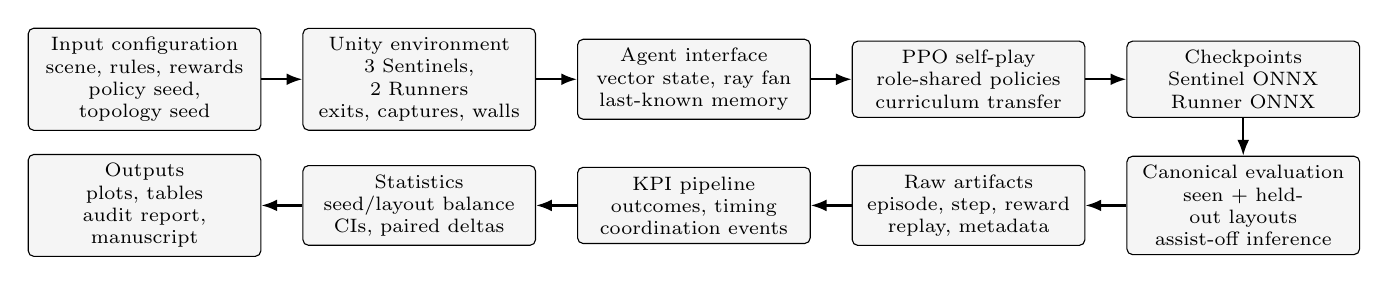
\begin{tikzpicture}[
font=\scriptsize,
node distance=0.48cm and 0.52cm,
block/.style={draw, rounded corners=2pt, align=center, minimum height=0.82cm, text width=2.28cm, fill=gray!8},
wideblock/.style={draw, rounded corners=2pt, align=center, minimum height=0.82cm, text width=2.72cm, fill=gray!8},
arrow/.style={-{Latex[length=2mm]}, thick}
]
\node[wideblock] (cfg) {Input configuration\\scene, rules, rewards\\policy seed, topology seed};
\node[wideblock, right=of cfg] (env) {Unity environment\\3 Sentinels, 2 Runners\\exits, captures, walls};
\node[wideblock, right=of env] (obs) {Agent interface\\vector state, ray fan\\last-known memory};
\node[wideblock, right=of obs] (train) {PPO self-play\\role-shared policies\\curriculum transfer};
\node[wideblock, right=of train] (ckpt) {Checkpoints\\Sentinel ONNX\\Runner ONNX};
\node[wideblock, below=of ckpt] (eval) {Canonical evaluation\\seen + held-out layouts\\assist-off inference};
\node[wideblock, left=of eval] (logs) {Raw artifacts\\episode, step, reward\\replay, metadata};
\node[wideblock, left=of logs] (kpi) {KPI pipeline\\outcomes, timing\\coordination events};
\node[wideblock, left=of kpi] (stats) {Statistics\\seed/layout balance\\CIs, paired deltas};
\node[wideblock, left=of stats] (paper) {Outputs\\plots, tables\\audit report, manuscript};

\draw[arrow] (cfg) -- (env);
\draw[arrow] (env) -- (obs);
\draw[arrow] (obs) -- (train);
\draw[arrow] (train) -- (ckpt);
\draw[arrow] (ckpt) -- (eval);
\draw[arrow] (eval) -- (logs);
\draw[arrow] (logs) -- (kpi);
\draw[arrow] (kpi) -- (stats);
\draw[arrow] (stats) -- (paper);
\end{tikzpicture}
\caption{Proposed methodology and evidence flow. The same seeded configuration controls training, evaluation, logging, KPI extraction, statistical analysis, and manuscript figures. Strict artifact validation excludes runs with missing logs, unknown seeds, or mismatched scene/rule/reward provenance from publication tables.}
\label{fig:methodology_flow}
\end{figure*}

Figure~\ref{fig:methodology_flow} summarizes the complete workflow. The core design choice is that simulation, learning, evaluation, and reporting are not treated as separate manual steps. Instead, every paper result is generated from run-scoped artifacts and auditable metadata. This is intended to reduce the common MARL failure mode in which training curves, screenshots, and hand-selected demonstrations cannot be traced back to reproducible seeds and configurations.

\subsection{Environment Structure}

The implementation includes four scenes of increasing complexity:
\begin{itemize}
    \item \textbf{Open arena baseline:} flat arena with no walls.
    \item \textbf{Static maze:} a fixed corridor topology with configurable placements.
    \item \textbf{Dynamic maze:} walls shift at configurable intervals during episodes.
    \item \textbf{Unseen evaluation maze:} novel layouts not encountered during training.
\end{itemize}

The dynamic maze is the core environment. Training uses a fixed base topology, while held-out evaluation topologies are generated deterministically from reserved seeds. In both cases, selected wall pillars can rise or lower on a timer. These shifts invalidate a fixed route during an episode and create trapping opportunities and escape adaptations in real time. Exit zones are placed explicitly for the Runner side, making evasion a goal-directed navigation task rather than pure survival.

\subsection{Seeded Topology Generation}

Held-out mazes use a $13\times13$ occupancy grid containing a $6\times6$ lattice of candidate free cells. A seeded randomized depth-first search carves a spanning tree $E_{\mathrm{tree}}$ over all 36 cells. Four additional non-tree connections are opened permanently to reduce single-corridor degeneracy, and up to five further non-tree connections are marked as dynamic wall edges. The traversable graph is therefore
\begin{equation}
E_t=E_{\mathrm{tree}}\cup E_{\mathrm{loop}}\cup E_{\mathrm{dyn}}(t),
\qquad E_{\mathrm{dyn}}(t)\subseteq E_{\mathrm{optional}}.
\end{equation}
Because $E_{\mathrm{tree}}$ is never removed, every generated topology remains connected even when all dynamic connections are raised. This is a construction-level safety property, not an empirical assumption. The reserved topology seeds are 101, 202, 303, 404, and 505. Topology seed $q_l$ is fixed within policy-layout cell $l$, whereas placement seed $q_l+k$ varies with episode $k$. Each episode row records both \texttt{maze\_layout\_id} and \texttt{maze\_topology\_seed}; this prevents placement randomization from being mislabeled as topology diversity.

\subsection{Agent Architecture}

The codebase separates agent logic, environment control, reward computation, sensing, and logging into distinct modules. \texttt{BaseAgent} handles movement, observation collection, and ML-Agents integration. \texttt{SentinelAgent} extends it with capture-radius logic and target tracking. \texttt{RunnerAgent} extends it with escape and captured-state management. The central \texttt{PursuitEvasionEnvController} manages episode lifecycle, capture detection, reward triggering, and terminal conditions.

The controller can optionally blend a learned direction $a_{i,t}$ with a geometric direction $h_{i,t}$:
\begin{align}
\widetilde{a}_{i,t}&=(1-\alpha_{i,t})a_{i,t}+\alpha_{i,t}h_{i,t},\\
\alpha_{i,t}&=\operatorname{clip}\!\left(\rho_q[c_q+(1-c_q)u_{i,t}],0,1\right).
\end{align}
where $q$ is the role, $\rho_q$ is the configured assist strength, and $u_{i,t}$ increases as the visible or remembered target becomes nearer. The source uses $c_S=0.35$ for pursuit and $c_R=0.30$ for evasion, with obstacle-aware sliding applied to $h_{i,t}$. Training uses $\rho_S=0.15$ and $\rho_R=0$, but the canonical publication evaluation sets both to zero so reported policy behavior is unassisted. Since $h_{i,t}$ is computed outside the policy network, the matched assist-on intervention reinstates $\rho_S=0.15$ and measures a hybrid controller while retaining the checkpoint, topology, placements, and every other rule parameter.

\subsection{Observation Design}

The observation pipeline is state-based rather than camera-based. Table~\ref{tab:state_action} shows the complete breakdown. Each agent receives a flat vector containing self-state (position, velocity, heading, alive flag), environment context (time remaining, nearest exit distance and direction, wall proximity, wall shift timer), a fixed-height 360-degree planar horizontal ray fan, last-known-position memory for targets that have left line of sight, and a summary of the two nearest opponents including their relative position, visibility, and threat pressure.

Sentinels cast 14 rays while Runners cast 16 rays. Each ray produces 6 floats: normalized hit distance and one-hot indicators for wall, exit, teammate, opponent, and other object types. This gives Runners wider sensing coverage because their survival depends on detecting threats from all directions.

\begin{table}[t]
\centering
\caption{Observation and action space per agent role.}
\label{tab:state_action}
\begin{tabular}{lcc}
\toprule
Component & Sentinel & Runner \\
\midrule
Self state & 10 & 10 \\
Environment context & 7 & 7 \\
Ray perception (6 per ray) & 84 (14 rays) & 96 (16 rays) \\
Last-known-position memory & 6 & 6 \\
Opponent summary (2 nearest) & 10 & 10 \\
\midrule
\textbf{Total observation size} & \textbf{117} & \textbf{129} \\
\midrule
Action space & 2 continuous & 2 continuous \\
\bottomrule
\end{tabular}
\end{table}

\subsection{Reward Design}

The reward system uses the \texttt{v5\_active\_agents} configuration, which was iteratively developed to address three behavioral failure modes observed during training: (1)~free-rider collapse, where one Sentinel learns to capture while others idle; (2)~cluster convergence, where all Sentinels chase the same Runner in a single file; and (3)~passive evasion, where Runners survive by standing still rather than actively seeking exits.

The reward function combines terminal win/loss signals with individual distance-based shaping for pursuit and evasion \cite{sheikh2020combined}, anti-clustering penalties, idle penalties, exit-seeking shaping, and a tactical coordination layer that rewards events detected by a dedicated \texttt{TrapEventDetector} module. The tactical layer rewards pincer formations, corridor control, exit denial, and dead-end forcing. All weights are loaded from YAML configuration files at runtime. Table~\ref{tab:rewards} lists the final reward weights.

For agent $i$, the implemented per-step reward can be written as
\begin{equation}
r_{i,t}=r^{\mathrm{terminal}}_{i,t}+\sum_{k\in\mathcal{D}}w_{i,k}\,g_k(\Delta d_{k,t})+
\sum_{m\in\mathcal{E}}w_{i,m}\,\phi_m(s_t,\mathbf{a}_t),
\end{equation}
where $\mathcal{D}$ contains distance-progress terms and $\mathcal{E}$ contains discrete behavioral and tactical events. For a target distance $d_t$, the shaping gate is
\begin{equation}
g(\Delta d_t)=\mathbb{1}(|\Delta d_t|>\delta)
\min\left(1,\frac{|\Delta d_t|}{\kappa}\right),
\end{equation}
with the sign and coefficient selected by whether the change is desirable. Sentinel chase progress uses $\Delta d_t=d_{t-1}-d_t$; Runner evasion uses $\Delta d_t=d_t-d_{t-1}$ while inside a configured threat radius; exit approach again uses $d_{t-1}-d_t$. The source defaults use a $0.08$ movement dead-zone for pursuit/evasion and $0.05$ for exit approach.

The shaping terms are not proven potential-based and may therefore change the optimal policy, not merely accelerate learning. This is a deliberate engineering tradeoff, but it makes reward ablation essential. We evaluate outcomes separately from shaped return so that an increase in accumulated shaping reward cannot be mistaken for improved capture or escape behavior.

\begin{table}[t]
\centering
\caption{Reward weights (\texttt{v5\_active\_agents} configuration).}
\label{tab:rewards}
\begin{tabular}{lc}
\toprule
\textbf{Sentinel Rewards} & Weight \\
\midrule
Team full capture (win) & $+1.0$ \\
Timeout or escape (loss) & $-1.0$ \\
Individual capture bonus & $+0.25$ \\
Chase progress (per step) & $+0.004$ \\
Chase regression & $-0.003$ \\
Cluster penalty & $-0.015$ \\
Idle penalty & $-0.002$ \\
Wall loop penalty & $-0.002$ \\
Exploration visit bonus & $+0.001$ \\
Orbit stall penalty & $-0.003$ \\
\midrule
\textbf{Runner Rewards} & Weight \\
\midrule
Team exit success (win) & $+1.0$ \\
Both captured (loss) & $-1.0$ \\
Tagged individually & $-0.2$ \\
Survival step bonus & $+0.0001$ \\
Exit approach bonus & $+0.005$ \\
Exit approach regression & $-0.002$ \\
Evade progress & $+0.001$ \\
Threat approach penalty & $-0.002$ \\
Wall loop penalty & $-0.001$ \\
Exploration visit bonus & $+0.001$ \\
Orbit stall penalty & $-0.003$ \\
\bottomrule
\end{tabular}
\end{table}

\subsection{Logging and Reproducibility}

Each training and evaluation run produces four CSV artifacts under a run-specific directory: \texttt{episode\_log.csv} (per-episode outcomes and totals), \texttt{agent\_step\_log.csv} (per-step positions, actions, and distances), \texttt{reward\_audit.csv} (per-event reward attribution by agent, category, and magnitude), and \texttt{replay\_events.csv} (timestamped capture, escape, wall-shift, and tactical events). This structure ties every reported metric back to raw per-step evidence.

The Python launcher writes a second provenance layer containing the run manifest, seed, exact training or inference command, Git state, configuration snapshots, and SHA-256 hashes. Unity receives the repository root and requested scene through explicit environment variables; runtime override files select curriculum, rule, and reward configurations. Episode rows repeat the effective scene and configuration names, allowing the audit to compare requested and observed provenance rather than trusting launcher metadata alone.

A run is publication-valid only when all required artifacts are non-empty, the seed and run identifier are known, at least one episode is complete, and the observed scene/rule/reward tuple matches the manifest. This strictness detected an earlier 18-cell matrix in which the standalone silently loaded its default scene and configuration. That matrix is retained with an \texttt{INVALIDATED.md} marker but excluded from every reported result. The failure case demonstrates why artifact existence without semantic provenance is insufficient.

The same rule applies to retries. ML-Agents \texttt{--force} replaces trainer outputs but does not truncate CSV files written independently by Unity. A corrected training retry was therefore stopped when its V5 rows were found appended to legacy reward rows. The launcher now deletes the complete target run directory before a forced launch and writes an explicit \texttt{running} status before starting Unity. The mixed directory is preserved as invalidated audit evidence, never as a source of checkpoints or results.

\begin{table}[t]
\centering
\caption{Reviewer-facing artifact map in the public repository.}
\label{tab:artifact_map}
\scriptsize
\setlength{\tabcolsep}{3pt}
\begin{tabular}{p{2.7cm}p{4.4cm}}
\toprule
Artifact & Purpose \\
\midrule
Unity scripts & Agent control, sensing, reward logic, episode lifecycle, and CSV logging implementation \\
Configuration files & Trainer, reward, rule, curriculum, ablation, and evaluation manifests \\
Setup validator & Environment and repository preflight checks before experiments \\
Policy evaluator & Fixed-checkpoint inference launcher with metadata and log routing \\
Readiness auditor & Gate-level audit for manuscript, training, evaluation, ablation, and reproducibility status \\
Unit tests & Evaluation isolation and publication metric calculations \\
Evaluation summaries & Canonical assist-off 30-cell evaluation summaries and statistics \\
Official summaries & Learning curves, paired ablations, readiness reports, and power analysis outputs \\
\bottomrule
\end{tabular}
\end{table}

% ============================================================
\section{Training and Evaluation Setup}
% ============================================================

\subsection{Training Algorithm}

We train both behaviors with PPO using parameter sharing within each team and asymmetric self-play across teams. All three Sentinels share a single policy network, and both Runners share a separate one. Table~\ref{tab:hyperparams} lists the official maze-stage hyperparameters. The excluded legacy open-arena trainer used a 1024 batch and a 64-step horizon and is not part of the four-stage official matrix. The learning rate follows a linear decay schedule over the training run. A draft MA-POCA YAML exists, but it is not a valid matched baseline: team-group registration, equalized budgets, self-play controls, and independent validation remain to be implemented. No MA-POCA result or support claim is made here.

For role $q$, let $r_t(\theta_q)=\pi_{\theta_q}(a_t\mid o_t)/\pi_{\theta_q^{\mathrm{old}}}(a_t\mid o_t)$ and let $\widehat{A}_{q,t}$ be the generalized advantage estimate. The policy term optimized by PPO is
\begin{align}
L_q^{\mathrm{clip}}(\theta_q)=\mathbb{E}_t\big[\min\big(&r_t(\theta_q)\widehat{A}_{q,t},\nonumber\\
&\operatorname{clip}(r_t(\theta_q),1-\epsilon,1+\epsilon)\widehat{A}_{q,t}\big)\big].
\end{align}
The implementation combines this term with a value loss and entropy bonus. This objective is applied independently to the Sentinel and Runner parameter sets; it does not centralize the critic across opposing roles. Checkpoint transfer initializes both $\theta_S$ and $\theta_R$ at the next curriculum stage, while optimizer progress and the new stage budget are recorded in run metadata.

\begin{table}[t]
\centering
\caption{PPO hyperparameters (shared by both behaviors).}
\label{tab:hyperparams}
\begin{tabular}{lcc}
\toprule
Parameter & Static Maze & Dynamic Maze \\
\midrule
Learning rate & $3.0{\times}10^{-4}$ & $2.5{\times}10^{-4}$ \\
Batch size & 2048 & 2048 \\
Buffer size & 20480 & 40960 \\
Entropy ($\beta$) & $5.0{\times}10^{-3}$ & $4.0{\times}10^{-3}$ \\
Clip range ($\epsilon$) & 0.2 & 0.2 \\
GAE $\lambda$ & 0.95 & 0.95 \\
Discount ($\gamma$) & 0.99 & 0.99 \\
Epochs per update & 3 & 4 \\
Hidden units & 256 & 256 \\
Hidden layers & 2 & 2 \\
Time horizon & 128 & 160 \\
Sentinel max steps & 1{,}500{,}000 & 1{,}500{,}000 \\
Runner max steps & 1{,}500{,}000 & 1{,}500{,}000 \\
\bottomrule
\end{tabular}
\end{table}

\subsection{Curriculum and Transfer Learning}

Training follows a four-stage curriculum with transfer learning, motivated by evidence that staged difficulty helps agents discover coordination skills that are hard to learn from sparse reward alone \cite{grupen2021,zhang2023curriculum}. Each stage uses \texttt{--initialize-from} to bootstrap both role policies from the previous stage's checkpoint. The network architecture (256 hidden units, 2 layers) remains identical across stages so the parameter tensors are compatible.

Table~\ref{tab:curriculum} reports the implemented progression from the canonical curriculum YAML. Stage~1 uses a fixed static maze and fixed spawn/exit locations. Stage~2 randomizes spawn and exit locations in the same maze family. Stage~3 introduces one wall shift every 20 seconds. Stage~4 increases the shift frequency to 8 seconds, raises shift intensity from one to three wall changes, and changes the training maze seed from 42 to 84. This is more precise than describing the legacy open-arena plot as the official curriculum.

All four stages use the same \texttt{reward\_v5\_active\_agents} definition. A partial 590-episode Stage~1 run was invalidated when an audit found that earlier manifests switched reward definitions between static and dynamic stages; such a switch would confound curriculum difficulty with reward design. Its first V5 retry was also invalidated because old and new append-only logs shared a run directory. Under simultaneous training, equal limits then froze the faster-accumulating three-agent Sentinel trainer before Runner finished. A 3:2-budget retry avoided that timing error but was also excluded: Sentinel wins fell from 92\% in its first 100 episodes to 8\% in its last 100 episodes, evidence of latest-policy cycling rather than stable improvement. Opponent-snapshot self-play corrected the simultaneous-update design, but a source-level audit showed that retaining 3:2 limits would instead create a final 500k Sentinel-only tail under the ghost controller's equal-step turns; that partial run was also invalidated. The final configuration combines snapshot self-play with equal per-policy sample limits. The launcher refuses official training unless reward, clean-retry, role-budget, and self-play audits pass.

ML-Agents counts one wrapped-trainer step for each acting-agent transition. Its ghost controller changes the learning team after an equal number of wrapped-trainer steps and is designed to give every team the same trainer-step count. We therefore use 1.5M transition samples for each role per stage, so both optimizers receive equal sample budgets and finish self-play together. With role-level parameter sharing, these samples correspond to 0.5M Sentinel team decision cycles and 0.75M Runner team decision cycles because three Sentinels act per cycle but only two Runners do; we disclose both units rather than calling them equivalent. The matched direct-dynamic control uses 6M samples per role, exactly the aggregate four-stage curriculum budget.

\begin{table}[t]
\centering
\caption{Implemented four-stage curriculum. Step budgets are Sentinel/Runner trainer steps.}
\label{tab:curriculum}
\begin{tabular}{p{2.0cm}p{1.7cm}p{1.45cm}p{1.35cm}}
\toprule
Stage & Topology & Steps & Transfer \\
\midrule
1. Static fixed & Static, seed 42 & 1.5M/1.5M & -- \\
2. Static random & Static, seed 42 & 1.5M/1.5M & Stage 1 \\
3. Dynamic low & 20 s, intensity 1 & 1.5M/1.5M & Stage 2 \\
4. Dynamic high & 8 s, intensity 3 & 1.5M/1.5M & Stage 3 \\
\midrule
\textit{Evaluation} & Seen + 5 held out & -- & Stage 4 \\
\bottomrule
\end{tabular}
\end{table}

\subsection{Evaluation Protocol}

We evaluate trained policies in inference mode using fixed ONNX checkpoints. The strengthened publication protocol uses five policy seeds (42, 101, 202, 606, 707), one seen dynamic-maze split, and at least five held-out unseen layout seeds (101, 202, 303, 404, 505). Each policy-layout cell targets 100 completed episodes; a 30-minute wall-clock cap is a failure timeout rather than the sampling unit. All evaluation runs use deterministic action selection with seeded spawn/episode randomization and must produce run-scoped raw logs: \texttt{episode\_log.csv}, \texttt{agent\_step\_log.csv}, \texttt{reward\_audit.csv}, and \texttt{replay\_events.csv}. A run is excluded from publication tables if the episode target, any required log, metadata file, or KPI summary is missing.

The seen and held-out rule files are matched on agent speed, capture radius, timeout, wall-shift interval and intensity, sensing, zero action assistance, and all enabled randomization switches. Only the split identifier, topology seed, and placement/event seed differ. A machine-readable control audit compares the nested YAML fields before launch and rejects a matrix with any unregistered difference. The action-assist-on and dynamic-wall-off matrices use a parallel single-intervention audit: the former may change only the two assist coefficients, and the latter may change only \texttt{dynamic\_walls.enabled}.

The evaluation protocol reports outcome metrics (Sentinel win rate, Runner win rate, escape rate, survival time, and capture times), coordination metrics (pincer episode rate, trap frequency, corridor-block events, exit-denial events, Sentinel spread, and Runner separation), path metrics (path efficiency and route-change proxies after wall shifts), and ablation deltas. Primary results use zero action assistance; the paired assist-on matrix quantifies how much the optional hybrid controller changes those results.

\subsection{Metric Definitions}

For event type $m$, let $C_{k,m}$ be its count in episode $k$. We distinguish an episode prevalence from an event intensity:
\begin{equation}
\widehat{P}_m=\frac{1}{n}\sum_{k=1}^{n}\mathbb{1}[C_{k,m}>0],\qquad
\overline{C}_m=\frac{1}{n}\sum_{k=1}^{n}C_{k,m}.
\end{equation}
Calling both quantities a ``rate'' would be ambiguous, so exported summaries use names such as \texttt{pincer\_episode\_rate} and \texttt{pincer\_events\_per\_episode}. Trap success is conditional:
\begin{equation}
\widehat{P}_{\mathrm{trap\to win}}=
\frac{\sum_k\mathbb{1}[C_{k,\mathrm{trap}}>0\land y_k=S]}
{\sum_k\mathbb{1}[C_{k,\mathrm{trap}}>0]}.
\end{equation}

At step $t$, Sentinel spread is the mean pairwise distance among active Sentinels,
\begin{equation}
D_S(t)=\binom{|\mathcal{I}_S^t|}{2}^{-1}\sum_{i<j}\|x_i(t)-x_j(t)\|_2,
\end{equation}
with an analogous Runner separation $D_R(t)$. Each spread is averaged over snapshots within an episode and then equally across episodes. Path length is $L_i=\sum_t\|x_i(t)-x_i(t-1)\|_2$, with positions keyed by episode and agent so resets are not counted as motion. Capture times come from replay-event \texttt{time\_seconds}; Runner survival ends at that Runner's capture or at episode termination and is averaged over runner-episodes. For a wall shift at $\tau$ and one-second window $w$, route response is
\begin{equation}
\begin{aligned}
\theta_{j,\tau}&=\cos^{-1}\!\left(\frac{u^-\!\cdot u^+}{\|u^-\|\|u^+\|}\right),\\
u^-&=x_j(\tau)-x_j(\tau-w),\\
u^+&=x_j(\tau+w)-x_j(\tau).
\end{aligned}
\end{equation}
We report mean absolute deflection and the fraction with $\theta_{j,\tau}\ge45^\circ$; windows with less than 0.05~m displacement are excluded as directionally undefined.

\subsection{Statistical Analysis Plan}

The independent training seed is the unit of replication for policy-level claims. Episodes from the same checkpoint are not treated as independent policy replicates. We report each seed separately, then the mean and standard deviation across trained policies. Binary outcomes receive Wilson intervals within a policy/layout cell. For aggregate comparisons, a hierarchical bootstrap resamples policy seeds, then layouts, then episodes to preserve the nested design. Training uses the fixed \texttt{max\_steps} budgets in Table~\ref{tab:curriculum}; the YAML episode-count and win-rate thresholds are audited post hoc and do not terminate ML-Agents training.

Training curves are exported directly from each audited ML-Agents TensorBoard event file. Curves include cumulative reward, episode length, self-play ELO, entropy, policy loss, and value loss. They are aligned by role, curriculum stage, and normalized within-stage trainer progress; no run is admitted unless its completion audit passes. At every matched scalar step, the plot reports per-seed traces, the arithmetic mean, and a two-sided 95\% Student-$t$ interval across independent policy seeds. With five seeds the interval remains descriptive and potentially wide; smoothing is limited to the summary aggregation already performed by ML-Agents.

The full condition contains $5\times6\times100=3{,}000$ completed evaluation episodes. Applying the same budget to five ablations yields a planned minimum of 18,000 completed episodes after all retrained checkpoints are available. This count does not create 18,000 independent policy replicates: inference about training variability remains limited to five policy seeds. The larger within-cell count instead stabilizes per-topology outcome and timing estimates.

For metric observation $z_{s,l,k}$ from policy seed $s$, layout $l$, and episode $k$, the layout-balanced estimator is
\begin{equation}
\widehat{M}=\frac{1}{|\mathcal{S}|}\sum_{s\in\mathcal{S}}
\frac{1}{|\mathcal{L}|}\sum_{l\in\mathcal{L}}
\left(\frac{1}{n_{s,l}}\sum_{k=1}^{n_{s,l}}z_{s,l,k}\right).
\end{equation}
This prevents fast-terminating layouts from receiving more weight merely because they produce more episodes. The fixed-count protocol makes episode-weighted and layout-balanced estimates closer, but both are exported. Ablation effects are paired by training seed and evaluation layout:
\begin{equation}
\Delta_{a,s,l}=M_{\mathrm{full},s,l}-M_{a,s,l},
\end{equation}
where $a$ denotes an ablated component, $s$ a policy seed, and $l$ a layout. We report the mean paired effect, a 95\% bootstrap interval, and the raw per-seed values. With only five policy seeds, interval width and effect consistency matter more than a binary significance threshold.
For descriptive scale we also report the paired standardized effect
\begin{equation}
d_z=\overline{\Delta}_a/s(\Delta_a),
\end{equation}
along with the fraction of matched seed-topology cells having the modal effect sign. We retain the raw metric units because $d_z$ is unstable with a small policy-seed sample or when paired variance is near zero. The corresponding two-sided paired-$t$ power function is
\begin{equation}
\pi(d,n)=\Pr\!\left(\left|T_{n-1,\,d\sqrt{n}}\right|>
t_{1-\alpha/2,n-1}\right),
\end{equation}
where $T_{\nu,\lambda}$ is noncentral $t$. At $\alpha=0.05$, $n=5$, and 80\% power, numerical inversion gives $|d_z|\approx1.68$. Thus even five seeds detect only large effects: more episodes improve within-cell precision but not policy-level power, and a nonsignificant seed test is not evidence of no effect. The exported power audit also reports thresholds of 3.26 for three seeds and 1.00 for ten.

For outcome metric $M$, the topology generalization gap for policy seed $s$ is
\begin{equation}
G_s=M_{s,\mathrm{seen}}-\frac{1}{5}\sum_{l\in\mathcal{L}_{\mathrm{held}}}M_{s,l}.
\end{equation}
For Sentinel win rate, $G_s>0$ means Sentinel success decreases on held-out topologies; for Runner escape rate, $G_s>0$ means Runner escape success decreases. We state the role perspective for every gap rather than assigning one global ``favorable'' direction. We report the five held-out values alongside $G_s$ so that a favorable mean cannot hide a topology-specific failure. The statistics pipeline bootstraps each $G_s$ by resampling the seen episodes and then held-out layouts and their episodes. It also exports a balanced two-way decomposition of policy-seed, layout, and policy--layout-interaction-plus-cell-error variance from the cell means. No test treats the five layouts as five independently trained policies.

For held-out cell mean $\bar z_{s,l}$, the descriptive random-effects decomposition is
\begin{equation}
\bar z_{s,l}=\mu+a_s+b_l+u_{s,l},\qquad
\operatorname{Var}(\bar z)=\sigma_a^2+\sigma_b^2+\sigma_u^2,
\end{equation}
where $a_s$ is policy-seed variation, $b_l$ is layout variation, and $u_{s,l}$ combines seed--layout interaction with finite-cell estimation error. Method-of-moments components are truncated at zero and reported as variance fractions; with only five policy seeds they are descriptive rather than precise population estimates.

\begin{table*}[t]
\centering
\caption{Pre-registered ablation questions and acceptance evidence. Each condition uses policy seeds 42, 101, 202, 606, and 707 and the same held-out layouts.}
\label{tab:ablation_design}
\footnotesize
\begin{tabular}{p{2.5cm}p{3.4cm}p{4.1cm}p{4.0cm}}
\toprule
Ablation & Controlled change & Primary metrics & Interpretation \\
\midrule
Memory off & Retrain with the last-known-position subsystem disabled & Win/escape rate, capture time, reacquisition delay & Tests whether explicit system memory helps under occlusion \\
Tactical reward off & Retrain with trap/pincer/corridor/exit-denial rewards zeroed & Outcome rates and event prevalence/intensity & Separates coordination behavior from reward accounting \\
Dynamic walls off & Evaluate the same policies with matched topology/placement seeds & Survival, path length, route-change proxy & Measures the cost of within-episode topology changes \\
Direct dynamic training & Retrain without checkpoint transfer; match total environment steps & Learning curve, final outcome rates, seed variance & Tests the curriculum hypothesis \\
Action assist on & Evaluate the same policies with Sentinel pursuit blend restored to 0.15 & All outcome and coordination metrics & Quantifies non-policy control contribution relative to the canonical assist-off evaluation \\
\bottomrule
\end{tabular}
\end{table*}

Memory, tactical-reward, and curriculum ablations alter the learning problem and therefore require paired retraining for every policy seed. Dynamic-wall and action-assist ablations are deployment-time interventions on the same checkpoints; pairing the policy and episode/topology seeds isolates the immediate contribution of those mechanisms. We do not mix these two ablation types in one effect estimate.

The machine-readable suite pre-registers signs under the convention \emph{canonical full minus condition}: shorter reacquisition with memory, higher tactical-event prevalence with tactical shaping, a smaller absolute transfer gap after curriculum training, higher Sentinel win rate with assist on, and stronger route deflection with dynamic walls. Metrics outside these hypotheses are explicitly exploratory; disagreement with a registered sign is reported as a negative result rather than relabeled post hoc.

The memory intervention is a system-level ablation rather than a neural-input-only mask. It writes zeros into the fixed six-dimensional memory observation, stops last-known-target updates, and prevents the pursuit-assist controller from falling back to a remembered target when no opponent is visible. This preserves observation dimensionality and network compatibility, but any measured effect must be attributed to the complete explicit-memory subsystem.

% ============================================================
\section{Current Official Evidence at Pause}
% ============================================================

\noindent\textbf{Pause status.} The strengthened campaign was intentionally
paused on 2026-07-18 after completing the official curriculum baseline, the
canonical assist-off evaluation, and two deployment-time paired ablations. The
strict campaign tracker reported 47/65 training runs and 90/180 target-complete
evaluation cells. The publication-readiness audit passed 14/16 gates. The two
remaining blockers were official evaluation completeness for unfinished
ablation families and paired ablation completeness: only two of five planned
paired analyses were complete. Consequently, this section reports the
completed evidence honestly and does not claim completion of the full journal
experiment matrix.

The official five-seed curriculum baseline reached 20/20 audited training
runs. Figure~\ref{fig:official_training_reward} summarizes the exported
TensorBoard reward traces for the five independent policy seeds. The curve
export contains 28,320 scalar rows and is generated from
\texttt{results/official\_summary/training\_curves/}. It is an audited
learning-curve artifact, not a stopping criterion: all official stages use
fixed trainer step budgets.

\begin{figure}[t]
    \centering
    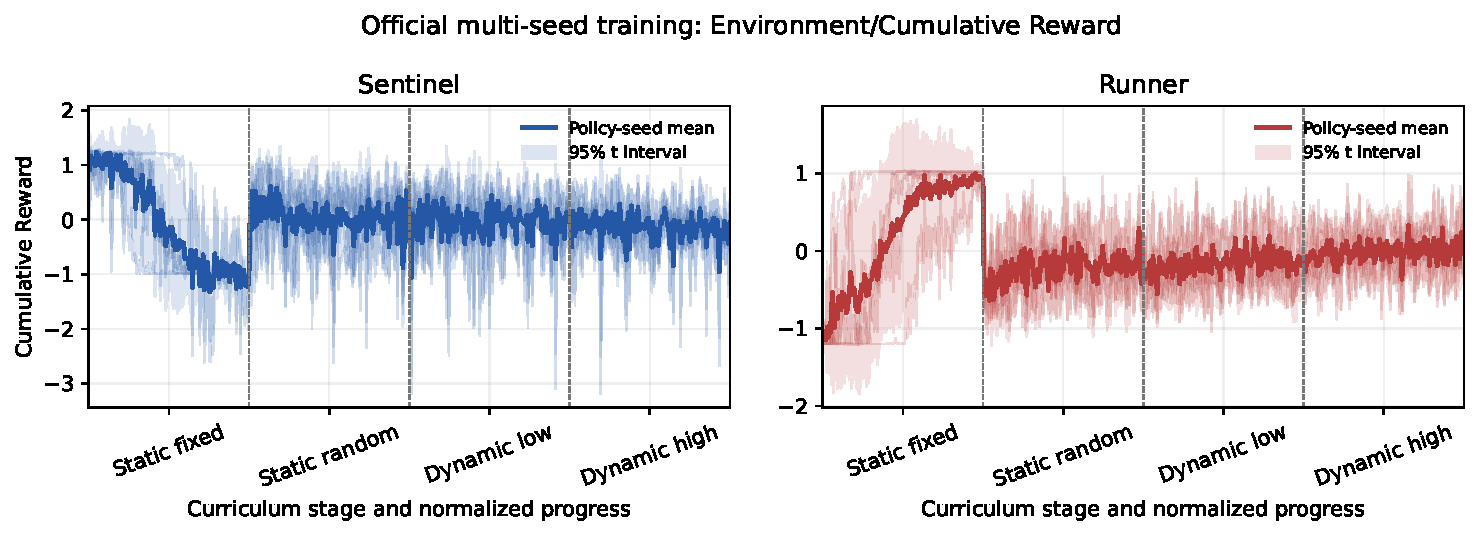
\includegraphics[width=0.48\textwidth]{fig_official_training_reward.pdf}
    \caption{Audited five-seed official curriculum reward curves exported from
    TensorBoard scalars. The official gate uses fixed trainer step budgets; the
    plotted curves are diagnostic summaries of completed training.}
    \label{fig:official_training_reward}
\end{figure}

Figure~\ref{fig:official_training_elo} reports the corresponding self-play ELO
traces. ELO is useful for detecting cycling and relative opponent difficulty,
but it is not treated as a game-theoretic equilibrium certificate.

\begin{figure}[t]
    \centering
    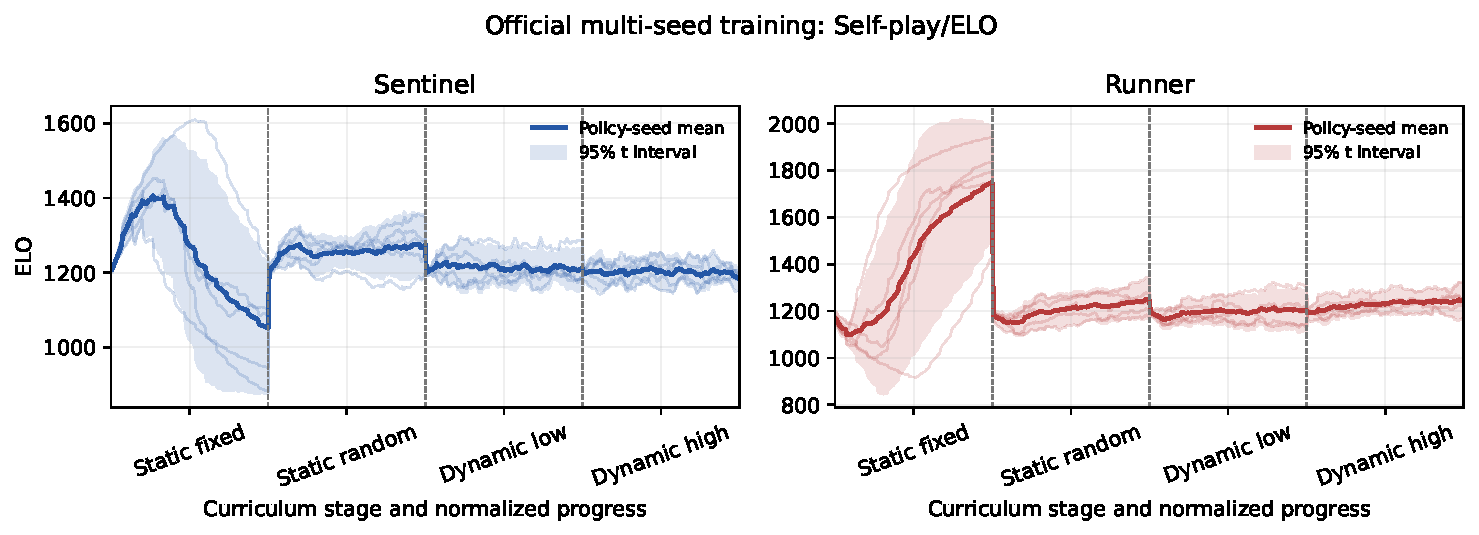
\includegraphics[width=0.48\textwidth]{fig_official_training_elo.pdf}
    \caption{Audited five-seed self-play ELO traces. Stable or increasing ELO
    does not imply Nash convergence; it is used as a training diagnostic.}
    \label{fig:official_training_elo}
\end{figure}

\subsection{Canonical Assist-Off Evaluation}

The canonical evaluation uses the five trained curriculum policy seeds
$(42,101,202,606,707)$, one seen topology, five held-out topologies, and a
target of 100 completed episodes per policy-topology cell. This yields 30
completed cells and 3,002 episodes because two cells slightly exceeded the
target before shutdown. Every reported row comes from the canonical evaluation
aggregate and passed the strict publication-evaluation audit.

\begin{table}[t]
\centering
\caption{Canonical assist-off evaluation over five policy seeds. Values are
means over policy-topology cells; the second number is the across-cell standard
deviation.}
\label{tab:official_eval_pause}
\footnotesize
\begin{tabular}{lcc}
\toprule
Metric & Seen & Five held-out topologies \\
\midrule
Cells / episodes & 5 / 501 & 25 / 2,501 \\
Sentinel win rate & 41.5\% $\pm$ 5.0 & 42.2\% $\pm$ 8.0 \\
Runner win rate & 58.5\% $\pm$ 5.0 & 57.8\% $\pm$ 8.0 \\
Escape rate & 52.9\% $\pm$ 7.4 & 53.5\% $\pm$ 9.5 \\
Full capture time & 23.70 $\pm$ 4.55 s & 22.79 $\pm$ 3.96 s \\
Pincer episode rate & 22.6\% $\pm$ 4.1 & 20.3\% $\pm$ 4.5 \\
Corridor block rate & 4.0\% $\pm$ 1.8 & 2.5\% $\pm$ 1.8 \\
Exit denial rate & 42.7\% $\pm$ 2.9 & 39.2\% $\pm$ 4.6 \\
Trap success rate & 49.4\% $\pm$ 4.2 & 50.4\% $\pm$ 8.0 \\
\bottomrule
\end{tabular}
\end{table}

Table~\ref{tab:official_eval_pause} changes the interpretation of the earlier
legacy story. Under canonical assist-off evaluation, the task is not
Sentinel-dominated. Runner wins are more common than Sentinel wins on both the
seen and held-out splits, and escapes account for roughly half of all episodes.
This is evidence of a playable asymmetric benchmark with meaningful evasion,
not evidence that the pursuer policy has solved the task. The held-out split is
not materially worse than the seen split at this aggregate level, but the
policy-seed variation is substantial: mean Sentinel win rate across the six
layouts ranges from 31.6\% for seed 101 to 50.8\% for seed 606. This is why the
paper reports per-seed results and avoids a robust-generalization claim.

\subsection{Completed Paired Ablations}

Two paired deployment-time interventions were complete at pause: action-assist
on/off and dynamic-wall on/off. The convention is canonical full condition
minus ablated condition. Thus, for \emph{action assist on}, a negative Sentinel
win delta means the canonical assist-off policy won less often than the
assist-on hybrid controller. For \emph{dynamic wall off}, a positive tactical
event delta means the dynamic-wall condition produced more of that event than
the static-wall intervention.

\begin{table}[t]
\centering
\caption{Completed paired ablations on held-out topologies at pause. Deltas use
the full-minus-condition convention and are paired by policy seed and topology.}
\label{tab:completed_ablations_pause}
\scriptsize
\setlength{\tabcolsep}{3pt}
\begin{tabular}{lrrrr}
\toprule
Ablation / metric & Delta & $d_z$ & Boot. low & Boot. high \\
\midrule
Assist on: Sentinel win & -1.26 pp & -0.17 & -6.88 pp & 4.44 pp \\
Assist on: escape & 1.82 pp & 0.25 & -3.64 pp & 7.38 pp \\
Assist on: Sentinel spread & -0.153 m & -0.48 & -0.290 & -0.011 \\
Assist on: pincer rate & 0.91 pp & 0.16 & -2.09 pp & 4.50 pp \\
\midrule
Wall off: Sentinel win & 2.06 pp & 0.29 & -2.74 pp & 7.22 pp \\
Wall off: pincer rate & 2.75 pp & 0.63 & 1.08 pp & 4.52 pp \\
Wall off: exit denial & 2.34 pp & 0.45 & 0.20 pp & 4.58 pp \\
Wall off: stall fraction & -6.46 pp & -1.21 & -8.77 pp & -3.77 pp \\
Wall off: trap episode rate & 3.16 pp & 0.76 & 1.08 pp & 5.40 pp \\
\bottomrule
\end{tabular}
\end{table}

The completed action-assist intervention does not show a reliable win-rate
benefit under the paired held-out analysis: the bootstrap interval spans zero.
It does, however, change some spatial behavior; canonical assist-off runs show
lower Sentinel spread under the full-minus-assist-on convention. This supports
disclosing assist settings but does not justify claiming that geometric
assistance is necessary for success.

The dynamic-wall intervention has clearer tactical effects. With dynamic walls
enabled, pincer episodes, exit denial, and trap episodes are higher on held-out
topologies, and stall-step fraction is lower. The Sentinel win-rate delta still
spans zero, so the defensible claim is behavioral: dynamic topology changes the
coordination-event profile more clearly than it changes terminal win rate in
the completed sample.

\subsection{Interpretability from Existing Artifacts}

The present manuscript does not report SHAP values or gradient saliency maps.
Instead, it provides three layers of model interpretation that can be generated
from the existing evidence pack. First, \texttt{reward\_audit.csv} identifies
which terminal, shaping, penalty, and tactical events contributed reward at
each episode stage. This makes it possible to separate a real outcome change
from a shaped-return increase. Second, \texttt{replay\_events.csv} exposes
behavioral mechanisms such as pincer pressure, corridor blocks, exit denial,
captures, escapes, and wall shifts. Third, the paired action-assist and
dynamic-wall interventions act as system-level counterfactual probes: the same
policy, topology seeds, and placement seeds are replayed while changing one
mechanism.

Under this interpretation lens, the current evidence is mixed and useful. The
assist-on probe does not show a reliable Sentinel win-rate gain, which weakens
any claim that the learned policy merely depends on geometric pursuit
assistance. The wall-off probe changes tactical-event prevalence more clearly
than terminal outcomes, suggesting that dynamic topology affects how agents
coordinate even when it does not yet produce a statistically clear win-rate
shift. This style of explanation is coarser than feature attribution, but it is
well matched to MARL: it interprets behavior at the event, team, and mechanism
levels where reviewers can connect policy outputs to pursuit-evasion concepts.
Future SHAP-style analysis should group inputs by semantic channels--self
state, wall rays, exit rays, opponent rays, teammate rays, memory, and time
context--rather than treating each scalar feature independently.

\subsection{Unfinished Evidence}

Three registered ablation families were not complete at pause: memory-off,
tactical-reward-off, and direct-dynamic training. Memory-off and tactical
reward ablations are retraining ablations, so they cannot be inferred from the
canonical checkpoints. Direct-dynamic is also a retraining condition and has the
largest remaining step budget. These incomplete gates are why the present PDF
should be used for advisor review or a workshop/preprint direction, not as a
final journal submission package.

% ============================================================
\section{Legacy Evidence Audit (Excluded from Official Results)}
% ============================================================

\noindent\textbf{Exclusion notice.} Every table and figure in this section is excluded from the official empirical study. The training plots use a legacy three-phase curriculum and legacy reward definitions. The fixed-checkpoint diagnostic executes a checkpoint named \texttt{v5\_dynamicmaze}, but its inference episodes load \texttt{reward\_dynamicmaze\_memory\_v4.yaml}, retain Sentinel action assistance at $\rho_S=0.15$, reuse one hard-coded unseen topology, and apply a compound rule shift. These artifacts validate execution and provenance tooling only; they do not answer RQ1--RQ3 and must be replaced by the registered v5 matrix.

\begin{table}[t]
\centering
\caption{Excluded legacy v4-era three-phase summary; historical motivation only.}
\label{tab:phase_results}
\begin{tabular}{lccc}
\toprule
Metric & Open+Static & Dynamic & Unseen \\
\midrule
Episodes & 3{,}228 & 2{,}492 & 30 \\
Sentinel win rate & 100.0\% & 66.8\% & 50.0\% \\
Runner win rate & 0.0\% & 33.2\% & 50.0\% \\
Sentinel mean reward & $+3.545$ & $+0.680$ & $+0.257$ \\
Runner mean reward & $-2.407$ & $-0.993$ & $-0.181$ \\
Wall-loop penalty & $-0.009$ & $-0.364$ & $-0.017$ \\
Cluster penalty & $-0.013$ & $-0.518$ & $-0.035$ \\
\bottomrule
\end{tabular}
\end{table}

The preliminary Sentinel win rate follows a curriculum-driven trend: near-perfect capture in the open arena/static maze setting, reduced dominance in the dynamic maze, and a balanced outcome in a small unseen-layout evaluation. We treat this as motivation rather than proof: stronger claims require repeated evaluation across policy seeds and multiple held-out layouts with confidence intervals.

\subsection{Validated Checkpoint Diagnostic}

After correcting standalone scene, rule-config, and reward-config routing, we evaluated the fixed \texttt{v5\_dynamicmaze} checkpoint pair across one seen layout and five held-out seed configurations. Despite the checkpoint name, episode provenance confirms that inference used the legacy v4 reward file; Table~\ref{tab:rewards} therefore does not describe this diagnostic. Three evaluation seeds were used, but these are not independent training seeds. Each matrix cell ran for 30 wall-clock seconds in deterministic inference mode. The audit accepted all 18 cells, all 108 required raw/KPI artifacts, and every episode-level scene/rule/reward provenance check. A subsequent code audit found two design confounds. First, the five configurations reused one hard-coded unseen topology; their seeds changed placements and stochastic events, not maze connectivity. Second, the legacy seen and unseen rule files changed agent speeds, capture radius, and wall timing together with the scene. They therefore measure transfer under a compound configuration shift, not a controlled topology effect.

\begin{table}[t]
\centering
\caption{Excluded assist-on/v4 fixed-checkpoint diagnostic. Intervals are 95\% Wilson intervals over completed episodes.}
\label{tab:validated_diagnostic}
\begin{tabular}{lcc}
\toprule
Metric & Seen & Five unseen configurations \\
\midrule
Completed episodes & 12 & 106 \\
Sentinel wins & 9 (75.0\%) & 73 (68.9\%) \\
95\% CI & [46.8, 91.1]\% & [59.5, 76.9]\% \\
Runner wins & 3 (25.0\%) & 33 (31.1\%) \\
Escape rate & 0.0\% & 25.5\% \\
Mean full capture time & 13.33 s & 21.04 s \\
\bottomrule
\end{tabular}
\end{table}

The aggregate result remains Sentinel-favored, but the seed configuration matters: Sentinel win rate ranges from 33.3\% under configuration 505 to 88.2\% under configuration 202. Because topology was shared, this variation cannot be attributed to maze geometry. The seen-versus-unseen difference also cannot be assigned to topology because agent and wall dynamics changed simultaneously. The diagnostic instead motivates controlled topology generation, matched rule parameters, fixed-count evaluation, and independently trained policy seeds.

The canonical statistics pipeline also computes equal-configuration estimates. For the five unseen configurations, the Sentinel win rate is 68.9\% when all 106 episodes are pooled and 68.3\% when every configuration receives equal weight. Mean full-capture time changes from 21.04~s to 23.25~s under equal weighting. Policy-level hierarchical intervals are deliberately omitted for this diagnostic because all rows share one checkpoint pair; nominal evaluation seeds do not create independent trained policies.

\begin{table}[t]
\centering
\caption{Excluded assist-on/v4 results on one shared unseen topology. ``Full cap.'' is mean full-capture time over Sentinel wins.}
\label{tab:per_layout}
\footnotesize
\begin{tabular}{lrrrrr}
\toprule
Configuration & $n$ & S wins & R wins & Esc. & Full cap. \\
\midrule
Seen 42 & 12 & 75.0\% & 25.0\% & 0.0\% & 13.33 s \\
Unseen 101 & 31 & 80.6\% & 19.4\% & 19.4\% & 22.04 s \\
Unseen 202 & 17 & 88.2\% & 11.8\% & 0.0\% & 14.23 s \\
Unseen 303 & 12 & 75.0\% & 25.0\% & 25.0\% & 58.67 s \\
Unseen 404 & 28 & 64.3\% & 35.7\% & 32.1\% & 9.63 s \\
Unseen 505 & 18 & 33.3\% & 66.7\% & 50.0\% & 11.68 s \\
\bottomrule
\end{tabular}
\end{table}

\subsection{What the Diagnostic Does and Does Not Establish}

The diagnostic is useful primarily as a test of executable transfer and measurement integrity. It establishes that the legacy ONNX pair runs in both requested scenes, that held-out rule files are actually loaded, and that complete episode, step, reward, replay, KPI, and metadata artifacts can be regenerated. It also identifies a concrete failure case: unseen seed 505 reverses the aggregate advantage and produces a 50\% escape rate.

It is not a controlled generalization experiment. First, all cells reuse one policy pair. Second, a fixed 30-second wall-clock budget produces unequal sample counts ($12$--$31$ episodes per configuration), so an episode-weighted aggregate gives greater influence to configurations with faster termination. Third, all unseen configurations reuse one topology, and deterministic inference makes nominal evaluation-seed repetitions partially redundant. Fourth, the legacy split comparison changes movement and wall parameters together with the scene. The official evaluation therefore uses a fixed completed-episode target per policy-topology cell, independent policy seeds, genuinely distinct seeded topologies, identical non-topology controls, and explicit spawn/episode randomization. Until those runs finish, Table~\ref{tab:per_layout} is a diagnostic table rather than the primary result of the paper.

\subsection{Reward Curves}

Figure~\ref{fig:reward_curves} shows the excluded legacy per-episode cumulative reward for both teams across the earlier three-phase curriculum. The green-shaded region corresponds to the open arena and static maze phases, where the Sentinel reward is consistently high ($+3.545$). The orange-shaded region marks the transition to the dynamic maze, where the Sentinel mean reward drops sharply to $+0.680$; this historical trace is not evidence for the official four-stage curriculum.

\begin{figure}[t]
    \centering
    
\includegraphics[width=0.48\textwidth]{fig_reward_curves.pdf}
    \caption{Excluded legacy three-phase cumulative reward; not comparable to the official v5 curriculum.}
    \label{fig:reward_curves}
\end{figure}

Figure~\ref{fig:reward_breakdown} decomposes the total reward into terminal, shaping, trap-aware, and penalty components. In the legacy run, terminal reward is the largest component, suggesting that shaping did not completely dominate win/loss learning. The publication pipeline verifies this claim by regenerating reward-breakdown tables from raw \texttt{reward\_audit.csv} files for every run.

\begin{figure}[t]
    \centering
    
\includegraphics[width=0.48\textwidth]{fig_reward_breakdown.pdf}
    \caption{Excluded legacy reward decomposition; not evidence about the official v5 weights.}
    \label{fig:reward_breakdown}
\end{figure}

\subsection{Win Rate Convergence}

Figure~\ref{fig:win_rate} shows the excluded legacy 100-episode rolling win rate for both teams. In the static maze phase, the Sentinel win rate is near 100\%. Upon entering the dynamic maze, the Runner win rate rises from near-zero toward a more balanced outcome. The trace motivates an evasion-viability hypothesis but cannot establish a dynamic-topology effect or equilibrium.

\begin{figure}[t]
    \centering
    
\includegraphics[width=0.48\textwidth]{fig_win_rate.pdf}
    \caption{Excluded legacy win-rate trace; descriptive history rather than an official comparison.}
    \label{fig:win_rate}
\end{figure}

\subsection{Penalty Reduction as Evidence of Learning}

Figure~\ref{fig:penalty_reduction} tracks penalty signals for both teams across training. The Sentinel cluster penalty, introduced to prevent free-rider collapse, shows that agents initially bunched together but gradually learned to spread out. The Runner threat-approach penalty decreases over training, indicating that Runners learned to maintain safe distances from Sentinels rather than passively waiting.

\begin{figure}[t]
    \centering
    
\includegraphics[width=0.48\textwidth]{fig_penalty_reduction.pdf}
    \caption{Excluded legacy penalty traces; not comparable to the official v5 reward definition.}
    \label{fig:penalty_reduction}
\end{figure}

\subsection{Shaping Signal Analysis}

Figure~\ref{fig:shaping} shows legacy distance-based shaping traces. Because the source runs predate the official v5 definition and the v4 diagnostic lacks the v5 idle and exit-approach terms, this plot cannot establish that v5 reduced passive evasion; it is retained only to document the hypothesis that motivated the registered reward ablation.

\begin{figure}[t]
    \centering
    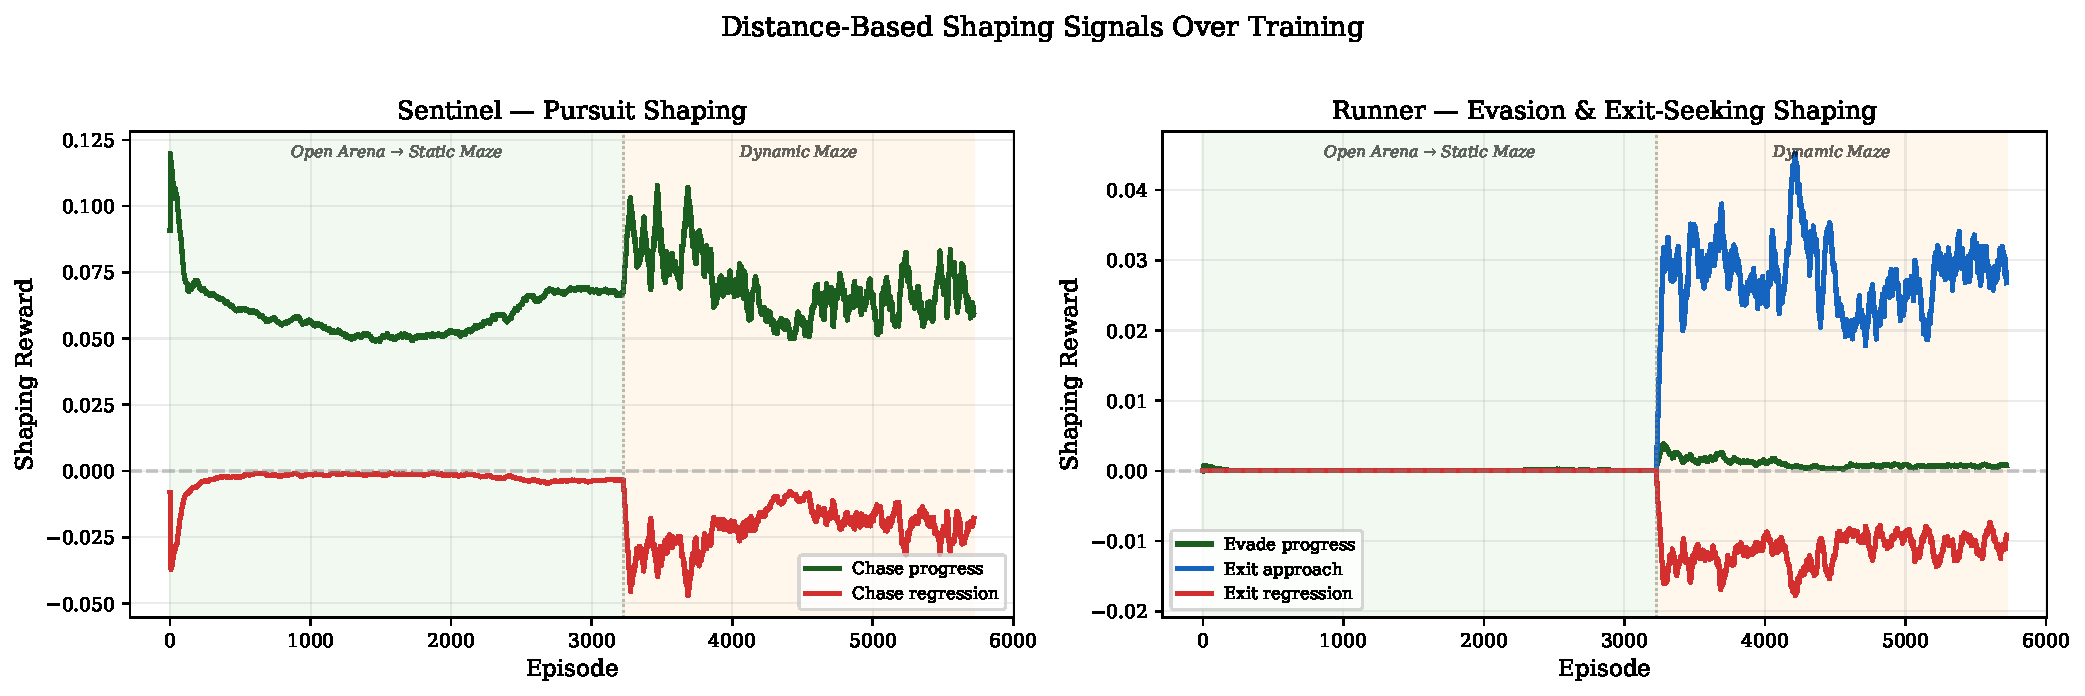
\includegraphics[width=0.48\textwidth]{fig_shaping_signals.pdf}
    \caption{Excluded legacy shaping traces; mechanism attribution requires the official tactical-reward ablation.}
    \label{fig:shaping}
\end{figure}

\subsection{Per-Phase Summary}

Figure~\ref{fig:phase_summary} presents the per-phase comparison as bar charts. The progression motivates a curriculum-learning hypothesis, but final zero-shot generalization claims require the expanded unseen-layout protocol.

\begin{figure}[t]
    \centering
    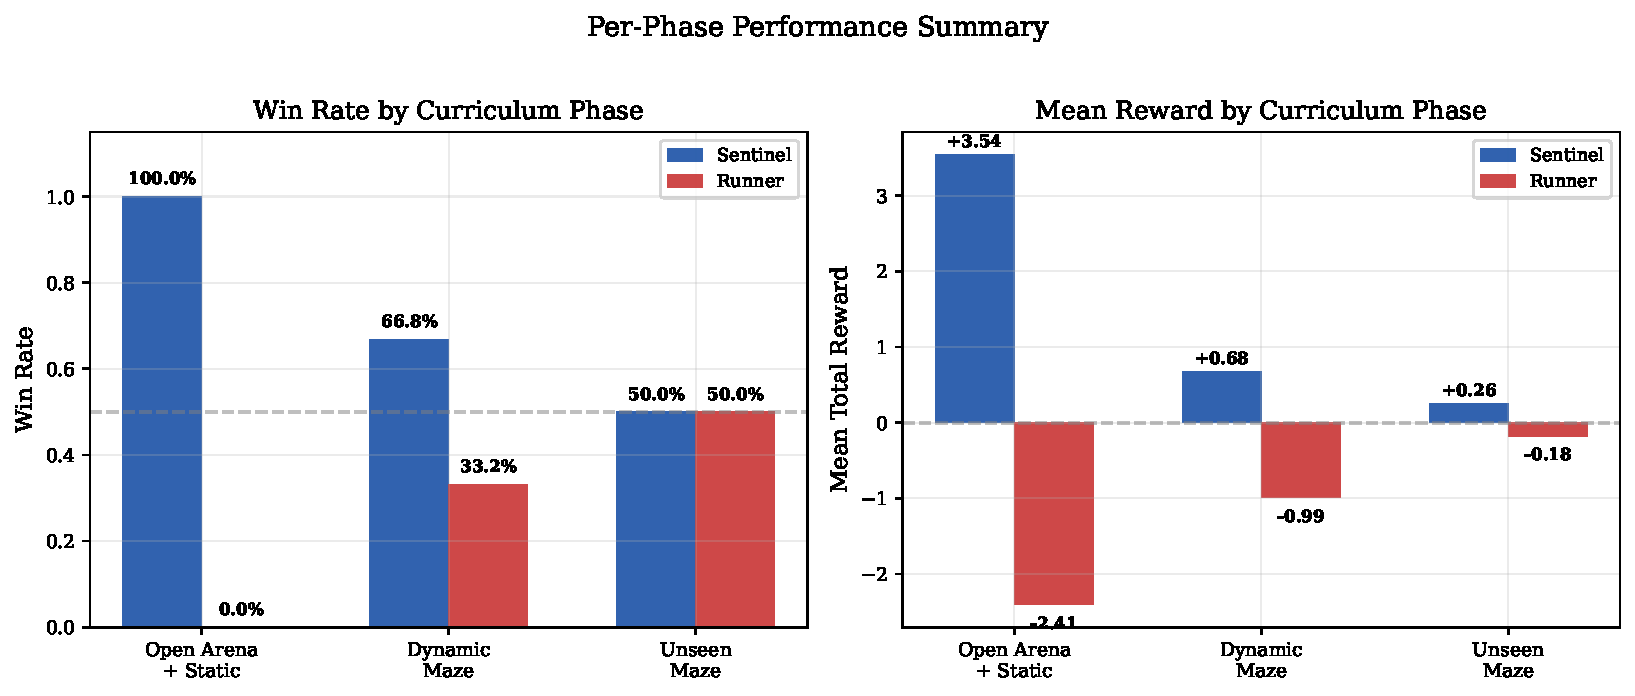
\includegraphics[width=0.48\textwidth]{fig_phase_summary.pdf}
    \caption{Excluded legacy phase summary; it motivates but does not test the curriculum hypothesis.}
    \label{fig:phase_summary}
\end{figure}

\subsection{Held-Out Configuration Diagnostic}

The validated diagnostic confirms that the dynamic-maze checkpoint can execute in the held-out scene with seed-specific rule and reward configurations. Across 106 completed unseen-scene episodes, the aggregate Sentinel win rate is 68.9\%, but the shared hard-coded topology means the 33.3--88.2\% spread is not a topology-generalization result. The upgraded generator now derives a connected maze from each held-out topology seed, separates topology seed from per-episode placement seed, and logs both the layout identifier and topology seed. The official experiment must rerun all five generated topologies with independently trained policies and fixed episode counts.

% ============================================================
\section{Discussion}
% ============================================================

The excluded audit motivates three hypotheses; it does not support completed findings.

\textbf{Curriculum learning is a central hypothesis.} The four-stage curriculum with transfer learning is designed to develop complex pursuit-evasion skills progressively. Its benefit is not established by the legacy traces and must be tested against direct dynamic-maze training with matched architecture and environment-step budget.

\textbf{Custom reward shaping targets specific failure modes.} The iterative development of the \texttt{v5\_active\_agents} reward configuration was driven by three observed failure modes:
\begin{itemize}
    \item \textit{Free-rider collapse:} In early training, one Sentinel learned to capture while others remained idle to collect the shared team reward. The \texttt{idle\_penalty} ($-0.002$/step) and increased \texttt{individual\_capture\_bonus} ($+0.25$) were added to reduce this behavior.
    \item \textit{Cluster convergence:} All three Sentinels would chase the same Runner in single file, making evasion trivial. The \texttt{cluster\_penalty} ($-0.015$) encourages spatial separation; publication results must quantify this through Sentinel spread and pincer/corridor metrics.
    \item \textit{Passive evasion:} Runners learned to survive by standing still, avoiding threat-approach penalties but never seeking exits. The \texttt{exit\_approach\_bonus} ($+0.005$) and \texttt{exit\_approach\_regression} ($-0.002$) were added to encourage goal-directed escape behaviour.
\end{itemize}

\textbf{Generalization remains the key empirical test.} The validated fixed-checkpoint diagnostic demonstrates executable transfer to a held-out scene under five seeded configurations, not five different topologies. The official protocol tests the upgraded procedural generator using independent policy seeds and five topology seeds, with topology identity recorded in every episode row.

Compared to MatrixWorld~\cite{matrixworld2023}, which provides a grid-based pursuit-evasion benchmark, Labyrinth Breach operates in continuous 3D space with asymmetric teams, dynamic walls, and exit-based objectives. Compared to ViPER~\cite{viper2025}, which focuses on visibility-based pursuit, our environment adds team coordination pressure through the 3v2 asymmetry and tactical reward terms.

% ============================================================
\section{Code, Data, and Reproducibility}
% ============================================================

The source repository contains the Unity project, ML-Agents trainer manifests, reward/rule/curriculum YAML files, Python launchers, audit scripts, unit tests, manuscript source, and generated summary artifacts. The public URL is given in the abstract footnote. The intended reproduction path is documented in \texttt{docs/reproducibility\_guide.md}: build the Unity \texttt{6000.0.40f1} standalone, run the prelaunch validation gates, resume the official curriculum/evaluation/ablation launchers, export KPI summaries, rerun readiness audits, and compile the paper. The Python environment is specified by \texttt{environment.yml} and \texttt{requirements.txt}; the core versions are Unity ML-Agents package \texttt{com.unity.ml-agents@4.0.0}, Python \texttt{3.10.12}, \texttt{mlagents==1.1.0}, and \texttt{torch==2.2.1}.

The current PDF is generated from the journal \LaTeX{} source under \texttt{paper/}. Official evaluation results are read from the publication-evaluation aggregate directory; learning curves and paired ablations are read from the official-summary directory. The codebase includes unit tests under \texttt{tests/}; the last local validation for the publication pipeline previously passed the repository test suite, and the final manuscript build in this revision was rendered twice with \texttt{pdflatex}. The evidence-pack builder \texttt{build\_publication\_evidence\_pack.py} creates a hashed archive with \texttt{artifact\_manifest.json} and \texttt{SHA256SUMS}, but it is intentionally blocked for a formal submission pack until all readiness gates pass. This prevents an incomplete ablation matrix from being packaged as final journal evidence.

No additional random-policy or heuristic-baseline result is claimed in this manuscript. The existing lightweight paired interventions are action-assist on/off and dynamic-wall on/off, both evaluated from fixed checkpoints without retraining. A true random or hand-coded heuristic baseline would require an additional evaluation harness in Unity so that its observations, episode targets, topology seeds, and logging schema match the learned-policy protocol.

% ============================================================
\section{Limitations and Future Work}
% ============================================================

Several limitations remain. First, the current study is simulation-only and does not include physical robot validation. Second, wall collision correctness under all dynamic shift configurations has not been exhaustively validated; rare edge cases during wall transitions could allow agents to clip through geometry. Third, the tactical reward shaping terms add complexity to the reward landscape and could be exploited in ways not yet detected. Fourth, the current architecture uses last-known-position memory rather than recurrent neural memory, which may limit performance in highly dynamic environments. Fifth, the controller includes optional action-assist blending; canonical results are assist-off and must be accompanied by the registered assist-on intervention.

% ============================================================
\section{Conclusion}
% ============================================================

We presented Labyrinth Breach, a reproducible Unity ML-Agents benchmark for asymmetric multi-agent pursuit-evasion with dynamic topology, partial observation, exit-directed evasion, and tactical reward shaping. Legacy results motivate curriculum and reward hypotheses, but final claims require the registered multi-seed evaluation and ablations. The environment, configurations, logging pipeline, and checkpoints are public for reproduction and extension.

\bibliographystyle{IEEEtran}
\IEEEtriggeratref{28}
% Balance the final page for the verified bibliography.
\begin{thebibliography}{99}

\bibitem{ai641projectdoc}
AI641 -- AI for Robotics, ``Projects,'' course handout, Project 2: Reinforcement Learning-based multi-agent pursuit-evasion.

\bibitem{lowe2017maddpg}
R. Lowe, Y. Wu, A. Tamar, J. Harb, P. Abbeel, and I. Mordatch,
``Multi-Agent Actor-Critic for Mixed Cooperative-Competitive Environments,''
in \textit{Advances in Neural Information Processing Systems}, 2017.

\bibitem{rashid2018qmix}
T. Rashid, M. Samvelyan, C. S. de Witt, G. Farquhar, J. Foerster, and S. Whiteson,
``QMIX: Monotonic Value Function Factorisation for Deep Multi-Agent Reinforcement Learning,''
\textit{Journal of Machine Learning Research}, vol. 21, no. 178, pp. 1--51, 2020.

\bibitem{yu2022mappo}
C. Yu et al.,
``The Surprising Effectiveness of PPO in Cooperative Multi-Agent Games,''
in \textit{Advances in Neural Information Processing Systems}, 2022.

\bibitem{verma2019mapel}
T. Verma, F. M. Zegers, and P. P. Khargonekar,
``Multi-Agent Pursuer-Evader Learning using Situation Report,''
arXiv preprint arXiv:1910.07780, 2019.

\bibitem{wang2020implicit}
M. Zhou, Z. Liu, P. Sui, Y. Li, and Y. Y. Chung,
``Learning Implicit Credit Assignment for Cooperative Multi-Agent Reinforcement Learning,''
in \textit{Advances in Neural Information Processing Systems}, 2020.

\bibitem{chen2023explicit}
W. Chen, W. Li, X. Liu, S. Yang, and Y. Gao,
``Learning Explicit Credit Assignment for Cooperative Multi-Agent Reinforcement Learning via Polarization Policy Gradient,''
in \textit{Proceedings of the AAAI Conference on Artificial Intelligence},
vol. 37, no. 10, pp. 11542--11550, 2023,
doi: 10.1609/aaai.v37i10.26364.

\bibitem{gonultas2024}
O. Gonultas and V. Isler,
``Learning to Play Pursuit-Evasion with Dynamic and Sensor Constraints,''
arXiv preprint arXiv:2405.05372, 2024.

\bibitem{matrixworld2023}
L. Sun, Y.-C. Chang, C. Lyu, C.-T. Lin, and Y. Shi,
``MatrixWorld: A Pursuit-Evasion Platform for Safe Multi-Agent Coordination and Autocurricula,''
arXiv preprint arXiv:2307.14854, 2023.

\bibitem{kouzeghar2023}
M. Kouzeghar, Y. Song, M. Meghjani, and R. Bouffanais,
``Multi-Target Pursuit by a Decentralized Heterogeneous UAV Swarm using Deep Multi-Agent Reinforcement Learning,''
in \textit{Proc. IEEE Int. Conf. Robot. Autom. (ICRA)}, 2023.

\bibitem{chen2023dualcl}
J. Chen, G. Li, C. Yu, X. Yang, B. Xu, H. Yang, and Y. Wang,
``A Dual Curriculum Learning Framework for Multi-UAV Pursuit-Evasion in Diverse Environments,''
arXiv preprint arXiv:2312.12255, 2023.

\bibitem{zheng2023encirclement}
Y. Zheng, Y. Zhang, C. Zhao, H. Yang, T. Li, Q. Ouyang, and Y. Chen,
``Faster Target Encirclement with Utilization of Obstacles via Multi-Agent Reinforcement Learning,''
in \textit{Proc. Asian Conf. Mach. Learn.}, PMLR, vol. 222, pp. 1731--1746, 2024.

\bibitem{viper2025}
Y. Wang, Y. Cao, J. Chiun, S. Koley, M. Pham, and G. A. Sartoretti,
``ViPER: Visibility-based Pursuit-Evasion via Reinforcement Learning,''
in \textit{Proceedings of the 8th Conference on Robot Learning}, PMLR, vol. 270, pp. 4188--4200, 2025.

\bibitem{lu2025epg}
R. Lu, P. Zhang, R. Shi, Y. Zhu, D. Zhao, Y. Liu, D. Wang, and C. Alippi,
``Equilibrium Policy Generalization: A Reinforcement Learning Framework for Cross-Graph Zero-Shot Generalization in Pursuit-Evasion Games,''
in \textit{Advances in Neural Information Processing Systems}, 2025.

\bibitem{lu2026r2ps}
R. Lu, R. Shi, Y. Zhu, and D. Zhao,
``R2PS: Worst-Case Robust Real-Time Pursuit Strategies under Partial Observability,''
in \textit{Proc. Int. Conf. Learn. Representations (ICLR)}, 2026.

\bibitem{yan2019uncertain}
F. Yan, J. Jiang, K. Di, Y. Jiang, and Z. Hao,
``Multiagent Pursuit-Evasion Problem with the Pursuers Moving at Uncertain Speeds,''
\textit{Journal of Intelligent \& Robotic Systems}, vol. 95, no. 1, pp. 119--135, 2019.

\bibitem{foerster2018coma}
J. Foerster, G. Farquhar, T. Afouras, V. Nardelli, and S. Whiteson,
``Counterfactual Multi-Agent Policy Gradients,''
in \textit{Proceedings of the AAAI Conference on Artificial Intelligence},
vol. 32, no. 1, pp. 2974--2982, 2018, doi: 10.1609/aaai.v32i1.11794.

\bibitem{zhang2023curriculum}
R. Bhati, S. K. Gottipati, C. Mars, and M. E. Taylor,
``Curriculum Learning for Cooperation in Multi-Agent Reinforcement Learning,''
in \textit{Second Agent Learning in Open-Endedness Workshop at NeurIPS}, 2023.

\bibitem{sheikh2020combined}
H. U. Sheikh and L. B\"ol\"oni,
``Multi-Agent Reinforcement Learning for Problems with Combined Individual and Team Reward,''
arXiv preprint arXiv:2003.10598, 2020.

\bibitem{liu2024uav}
Y. Zhang, M. Ding, J. Zhang, Q. Yang, G. Shi, M. Lu, and F. Jiang,
``Multi-UAV Pursuit-Evasion Gaming Based on PSO-M3DDPG Schemes,''
\textit{Complex \& Intelligent Systems}, vol. 10, pp. 6867--6883, 2024,
doi: 10.1007/s40747-024-01504-1.

\bibitem{du2021uav}
W. Du, T. Guo, J. Chen, B. Li, G. Zhu, and X. Cao,
``Cooperative Pursuit of Unauthorized UAVs in Urban Airspace via Multi-Agent Reinforcement Learning,''
\textit{Transportation Research Part C: Emerging Technologies}, vol. 128, Art. no. 103122, 2021,
doi: 10.1016/j.trc.2021.103122.

\bibitem{peng2025limited}
Z. Peng, G. Wu, B. Luo, and L. Wang,
``Multi-UAV Cooperative Pursuit Strategy with Limited Visual Field in Urban Airspace: A Multi-Agent Reinforcement Learning Approach,''
\textit{IEEE/CAA Journal of Automatica Sinica}, vol. 12, no. 7, pp. 1350--1367, 2025,
doi: 10.1109/JAS.2024.124965.

\bibitem{qu2026usv}
X. Qu, C. Li, Y. Jiang, F. Long, and R. Zhang,
``Cooperative Pursuit of Unmanned Surface Vehicles Using Multi-Agent Reinforcement Learning,''
\textit{Journal of Shanghai Jiaotong University (Science)}, vol. 31, pp. 187--194, 2026,
doi: 10.1007/s12204-025-2816-6.

\bibitem{xu2025emergent}
S. Xu and Z. Dang,
``Emergent Behaviors in Multiagent Pursuit Evasion Games within a Bounded 2D Grid World,''
\textit{Scientific Reports}, vol. 15, Art. no. 29376, 2025,
doi: 10.1038/s41598-025-15057-x.

\bibitem{cetin2024shap}
E. Cetin, C. Barrado, E. Salami, and E. Pastor,
``Analyzing Deep Reinforcement Learning Model Decisions with Shapley Additive Explanations for Counter Drone Operations,''
\textit{Applied Intelligence}, vol. 54, pp. 12095--12111, 2024,
doi: 10.1007/s10489-024-05733-2.

\bibitem{sheng2026xai}
L. Sheng, X. Chen, Z. Pan, F. Cai, and H. Chen,
``From Individual Decisions to Team Emergence: A Survey on Explainable Cooperative Multi-Agent Reinforcement Learning,''
\textit{Artificial Intelligence Review}, 2026,
doi: 10.1007/s10462-026-11598-3.

\bibitem{haeri2022emergent}
P. K. Sharma, E. Zaroukian, D. E. Asher, and B. Howell,
``Emergent Behaviors in Multi-Agent Target Acquisition,''
arXiv preprint arXiv:2212.07891, 2022.

\bibitem{desouza2020}
C. de Souza Jr., R. Newbury, A. Cosgun, P. Castillo, B. Vidolov, and D. Kuli\'{c},
``Decentralized Multi-Agent Pursuit using Deep Reinforcement Learning,''
\textit{IEEE Robotics and Automation Letters}, vol. 6, no. 3, pp. 4552--4559, 2021.

\bibitem{grupen2021}
N. A. Grupen, D. D. Lee, and B. Selman,
``Multi-Agent Curricula and Emergent Implicit Signaling,''
in \textit{Proceedings of the 20th International Conference on Autonomous Agents and MultiAgent Systems}, pp. 560--568, 2021.

\bibitem{gorsane2022}
R. Gorsane, O. Mahjoub, R. J. de Kock, R. Dubb, S. Singh, and A. Pretorius,
``Towards a Standardised Performance Evaluation Protocol for Cooperative MARL,''
in \textit{Advances in Neural Information Processing Systems}, vol. 35, pp. 5510--5521, 2022.

\bibitem{kapoor2024}
A. Kapoor, B. Freed, J. Schneider, and H. Choset,
``Assigning Credit with Partial Reward Decoupling in Multi-Agent Proximal Policy Optimization,''
in \textit{Proceedings of the Reinforcement Learning Conference}, 2024.

\bibitem{akinmolayan2026}
M. Akinmolayan, D. Josyula, and D. Casbeer,
``Adaptive Interception in Dynamic Domains: Exploration of Hybrid Reinforcement Learning in Pursuit-Evasion Tasks,''
\textit{Proceedings of the AAAI Spring Symposium Series}, vol. 8, no. 1,
pp. 2--10, 2026, doi: 10.1609/aaaiss.v8i1.42510.

\bibitem{zhao2025maca}
X. Zhao and Y. Xie,
``Multi-level Advantage Credit Assignment for Cooperative Multi-Agent Reinforcement Learning,''
in \textit{Proceedings of the 28th International Conference on Artificial Intelligence and Statistics}, PMLR, vol. 258, pp. 2971--2979, 2025.

\bibitem{zhao2026ma2mb}
B. Zhao, Q. Guo, X. Wang, R. Hedjam, and G. Zhong,
``MA2MB: Multi-Agent Mutual-Advising Model-Based Reinforcement Learning for Pursuit and Evasion Games,''
\textit{Robotics and Autonomous Systems}, vol. 203, Art. no. 105530, 2026.

\end{thebibliography}

\end{document}
